% !TEX root = saveliev_physics_general_course_1.tex
%!TEX TS-program = pdflatex
%!TEX encoding = UTF-8 Unicode


\chapter{CƠ HỌC CỦA VẬT RẮN}\label{chap:5}

\section{Chuyển động của một vật rắn}\label{sec:5_1}

%In Sec.~\ref{sec:1_1}, we acquainted ourselves with the two fundamental kinds of motion of a rigid body---translation and rotation.
Trong Mục~\ref{sec:1_1}, ta đã làm quen với hai dạng chuyển động cơ bản của vật rắn là chuyển động tịnh tiến và chuyển động quay.

%In translation, all the points of a body receive displacements equal in magnitude and direction during the same time interval. Consequently, the velocities and accelerations of all the points are identical at every moment of time. It is therefore sufficient to determine the motion of one of the points of a body (for example, of its centre of mass) to completely characterize the motion of the entire body.
Trong chuyển động tịnh tiến, tất cả các điểm của vật thu được các độ dời như nhau về độ lớn và về hướng trong cùng một khoảng thời gian, vì vậy các vận tốc và gia tốc của mọi điểm tại mỗi thời điểm đều giống nhau. Do đó để đặc trưng hoàn toàn chuyển động của cả vật thì chỉ cần xác định chuyển động của một điểm (chẳng hạn như khối tâm).

%In rotation, all the points of a rigid body move along circles whose centres are on a single straight line called the axis of rotation. To describe rotation, we must set the position of the axis of rotation in space and the angular velocity of the body at each moment of time.
Trong chuyển động quay tất cả các điểm của vật rắn chuyển động theo các đường tròn có tâm nằm trên cùng một đường thẳng gọi là trục quay. Để mô tả chuyển động quay cần biết vị trí của trục quay trong không gian và vận tốc góc của vật tại mỗi thời điểm.

%Any motion of a rigid body can be represented as the superposition of the two fundamental kinds of motion indicated above. We shall show this for plane motion, \ie, motion when all the points of a body move in parallel planes. An example of plane motion is the rolling of a cylinder along a plane (\fig{5_1}).
Mọi chuyển động của vật rắn đều có thể được biểu diễn dưới dạng chồng chập của hai kiểu chuyển động cơ bản được nêu ở trên. Chúng ta sẽ biểu diễn điều này trong chuyển động song phẳng, tức những chuyển động mà các điểm trên vật chỉ chuyển động trên các mặt phẳng song song. Ví dụ như chuyển động lăn của một hình trụ trên một mặt phẳng (\fig{5_1}).

\begin{figure}[!htb]
	\begin{minipage}[t]{0.5\linewidth}
		\begin{center}
			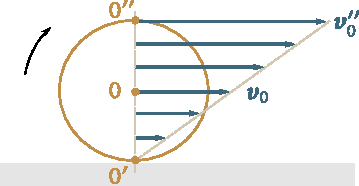
\includegraphics[scale=0.95]{figures/ch_05/fig_5_1.pdf}
			\caption[]{}
			\label{fig:5_1}
		\end{center}
	\end{minipage}
	\hspace{-0.05cm}
	\begin{minipage}[t]{0.5\linewidth}
		\begin{center}
			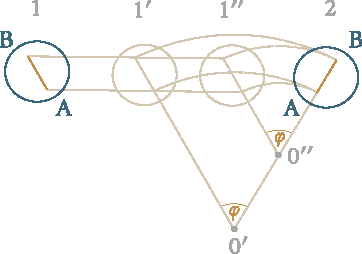
\includegraphics[scale=0.95]{figures/ch_05/fig_5_2.pdf}
			\caption[]{}
			\label{fig:5_2}
		\end{center}
	\end{minipage}
\end{figure}

%The arbitrary displacement of a rigid body from position $1$ to position $2$ (\fig{5_2}) can be represented as the sum of two displacements---translation from position $1$ to position $1'$ or $1''$, and rotation about the axis $0'$ or the axis $0''$. It is quite obvious that such a division of a displacement into translation and rotation can be performed in an infinite multitude of ways, but in any case rotation occurs through the same angle $\varphi$.
Độ dời bất kì của một vật rắn từ vị trí $1$ đến vị trí $2$ (\fig{5_2}) có thể được biểu diễn dưới dạng tổng của 2 độ dời---tịnh tiến từ vị trí $1$ đến $1'$ hoặc $1''$, và quay quanh trục $0$ hoặc trục $0'$. Dễ thấy rằng cách chia độ dời thành các thành phần tịnh tiến và quay có thể được thực hiện theo vô số cách khác nhau, tuy nhiên trong mọi trường hợp, phép quay được thực hiện theo cùng một góc $\varphi$ như nhau.

%In accordance with the above, the elementary displacement of a point of a body ds can be resolved into two displacements---the ``translational'' one $\deriv{\vec{s}}_{\text{tr}}$ and the ``rotational'' one $\deriv{\vec{s}}_{\text{rot}}$:
Ứng với điều ở trên, độ dời nguyên tố của một điểm trên vật rắn, $\deriv{\vec{s}}$ sẽ được tách thành hai phần---phần "tịnh tiến" $\deriv{\vec{s}}_{\text{tt}}$ và phần "quay" $\deriv{\vec{s}}_{\text{q}}$:
\begin{equation*}
\deriv{\vec{s}} = \deriv{\vec{s}}_{\text{tt}} + \deriv{\vec{s}}_{\text{q}}
\end{equation*}

\noindent
%where $\deriv{\vec{s}}_{\text{tr}}$ is the same for all the points of the body. This resolution of the displacement $\deriv{\vec{s}}$, as we have seen, can be performed in different ways. In each of them, the rotational displacement $\deriv{\vec{s}}_{\text{rot}}$ is performed by rotation of the body through the same angle $\deriv{\varphi}$ (but relative to different axes), whereas $\deriv{\vec{s}}_{\text{tr}}$ and $\deriv{\vec{s}}_{\text{rot}}$ are different.
trong đó $\deriv{\vec{s}}_{\text{tt}}$ đối với mọi điểm trên vật là như nhau. Như ta đã thấy, có thể tách độ dời $\deriv{\vec{s}}$ theo nhiều cách khác nhau, đồng thời trong mỗi cách, độ dời quay được thực hiện theo cùng một góc $\deriv{\varphi}$ (nhưng đối với các trục khác nhau) trong khi $\deriv{\vec{s}}_{\text{tt}}$ và $\deriv{\vec{s}}_{\text{q}}$ đều khác nhau.

%Dividing $\deriv{\vec{s}}$ by the corresponding time interval $\deriv{t}$, we get the velocity of a point:
Khi chia $\deriv{\vec{s}}$ cho khoảng thời gian tương ứng $\deriv{t}$ ta được vận tốc của một điểm:
%\begin{equation*}
%\vec{v} = \diff{\vec{s}}{t} = %\frac{\deriv{\vec{s}_{\text{tt}}}}{t} + %\frac{\deriv{\vec{s}_{\text{q}}}}{t} = \vec{v}_0 + %\vec{v}'
%\end{equation*}
\begin{equation*}
\vec{v} = \diff{\vec{s}}{t} = \diff{\vec{s}_{\text{tt}}}{t}+\diff{\vec{s}_{\text{q}}}{t}= \vec{v}_0 + \vec{v}'
\end{equation*}

\noindent
%where $\vec{v}_0$ is the velocity of translation, which is the same for all the points of a body, $\vec{v}'$ is the velocity due to rotation, which is different for different points of the body.
trong đó $\vec{v}_0$ là vận tốc tịnh tiến là như nhau với mọi điểm của vật, và $\vec{v}'$ là vật tốc gây ra bởi sự quay là khác nhau với những điểm khác nhau của vật.

%Thus, the plane motion of a rigid body can be represented as the sum of two motions---translation with the velocity $\vec{v}_0$ and rotation with the angular velocity $\vec{\omega}$ (the vector $\vec{\omega}$ in \fig{5_1} is directed at right angles to the plane of the drawing, beyond it). Such a representation of complex motion can be accomplished in many ways differing in the values of $\vec{v}_0$ and $\vec{v}'$, but corresponding to the same angular velocity $\vec{\omega}$. For example, the motion of a cylinder rolling without slipping along a plane (\fig{5_1}) can be represented either as translation with the velocity $\vec{v}_0$ and simultaneous rotation with the angular velocity $\vec{\omega}$ about the axis $0$, or as translation with the velocity $\vec{v}_0''=2\vec{v}_0$ and rotation with the same angular velocity $\vec{\omega}$ about the axis $0''$, or, finally, as only rotation, again with the same angular velocity $\vec{\omega}$ about the axis $0'$.
Như vậy, chuyển động song phẳng của một vật rắn có thể được biểu diễn là tổng của 2 chuyển động---tịnh tiến với vận tốc $\vec{v}_0$ và quay với vận tốc góc $\vec{\omega}$ (vector $\vec{\omega}$ trong \fig{5_1} nằm trên phương vuông góc với mặt phẳng của hình vẽ, hướng vào từ ngoài vào trong hình vẽ). Sự biểu diễn tương tự của một chuyển động phức tạp như vậy có thể thực hiện bằng nhiều cách khác nhau bởi các giá trị $\vec{v}_0$ và $\vec{v}'$ khác nhau, nhưng ứng với cùng một vận tốc góc $\vec{\omega}$. Chẳng hạn, có thể biểu diễn chuyển động của một hình trụ lăn không trượt theo một mặt phẳng (\fig{5_1}) như chuyển động tịnh tiến với vận tốc $\vec{v}_0$ và quay đồng thời với vận tốc góc $\vec{\omega}$ quanh trục $0$, hoặc như chuyển động tịnh tiến với vận tốc $\vec{v}_0''=2\vec{v}_0$ và quay với cùng vận tốc góc $\vec{\omega}$ quanh trục $0''$, hoặc, cuối cùng, như chỉ một chuyển động quay cũng cùng vận tốc góc $\vec{\omega}$ quanh trục $0'$.

%Assuming that the reference frame relative to which we are considering the complex motion of a rigid body is stationary, the motion of the body can be represented as rotation with the angular velocity $\vec{\omega}$ in a reference frame moving translationally with the velocity $\vec{v}_0$ relative to the stationary frame.
Giả sử rằng hệ quy chiếu mà đối với nó ta đang xét chuyển động phức tạp của vật rắn là đứng yên, thì có thể biểu diễn chuyển động của vật như sự quay với vận tốc góc $\vec{\omega}$ trong một hệ quy chiếu chuyển động tịnh tiến với vận tốc $\vec{v}_0$ đối với hệ đứng yên ban đầu.

%The linear velocity $\vec{v}'$ of a point with the position vector $\vec{r}$ due to rotation of a rigid body is $\vec{v}'=\vecprod{\omega}{r}$ [see~\eqn{1_100}]. Consequently, the velocity of this point in complex motion can be represented in the form
Vận tốc dài $\vec{v}'$ của một điểm có vector bán kính $\vec{r}$ do sự quay của vật rắn gây ra là $\vec{v}'=\vecprod{\omega}{r}$ (xem~\eqn{1_100}). Do đó, vận tốc của điểm này trong chuyển động phức tạp có thể biểu diễn dưới dạng
\begin{equation}\label{eq:5_1}
\vec{v} = \vec{v}_0 + \vecprod{\omega}{r}.
\end{equation}

%An elementary displacement of a rigid body in plane motion can always be represented as rotation about an axis called the \textbf{instantaneous axis of rotation}. This axis may be either inside the body or outside it. The position of the instantaneous axis of rotation relative to a fixed reference frame and relative to the body itself, generally speaking, changes with time. For a rolling cylinder (\fig{5_2}), the instantaneous axis $0'$ coincides with the line of contact of the cylinder with the plane. When the cylinder rolls, the instantaneous axis moves both along the plane (\ie, relative to a fixed reference frame) and along the surface of the cylinder.
Độ dời nguyên tố của một vật rắn trong chuyển động song phẳng luôn luôn có thể được biểu diễn như sự quay quanh một trục được gọi là \textbf{trục quay tức thời}. Trục này có thể nằm bên trong hay bên ngoài vật. Vị trí của trục quay tức thời đối với hệ quy chiếu đứng yên và đối với chính vật, nói chung, biến đổi theo thời gian. Trong trường hợp một hình trụ lăn (\fig{5_2}) trục tức thời $0'$ trùng với đường tiếp xúc của trụ và mặt phẳng. Khi hình trụ lăn, trục tức thời dịch chuyển vừa theo mặt phẳng (đối với hệ quy chiếu đứng yên) và vừa theo bề mặt hình trụ.

%The velocities of all the points of the body for each moment of time can be considered as due to rotation about the corresponding instantaneous axis. Consequently, plane motion of a rigid body can be considered as a number of consecutive elementary rotations about instantaneous axes.
Vận tốc của tất cả các điểm trên vật trong mọi thời điểm có thể được xem là gây ra bởi sự quay quanh một trục tức thời tương ứng. Do đó, có thể xét chuyển động song phẳng của vật rắn như một loạt phép quay liên tiếp xung quanh các trục tức thời.

%In non-planar motion, an elementary displacement of a body can be represented as rotation about an instantaneous axis only if the vectors $\vec{v}_0$ and $\vec{\omega}$ are mutually perpendicular. If the angle between these vectors differs from $\pi/2$, the motion of the body at each moment of time will be the superposition of two motions---rotation about a certain axis, and translation along this axis.
Trong chuyển động không song phẳng, độ dời nguyên tố của một vật chỉ có thể được biểu diễn như chuyển động quay quanh một trục tức thời nếu các vector $\vec{v}_0$ và $\vec{\omega}$ vuông góc với nhau. Nếu góc giữa các vector này khác $\pi/2$, chuyển động của vật ở mỗi thời điểm sẽ là chồng chập của hai chuyển động---quay quanh một trục nhất định, và tịnh tiến dọc theo trục này.

\section{Chuyển động của khối tâm vật rắn}\label{sec:5_2}

%By dividing a body into elementary masses $m_i$ we can represent it as a system of point particles whose mutual arrangement remains unchanged. Any of these elementary masses may be acted upon both by internal forces due to its interaction with other elementary masses of the body being considered, and by external forces. For example, if a body is in the field of the Earth's gravitational forces, each elementary mass of the body $m_i$ will experience an external force equal to $m\vec{g}$.
Bằng cách chia nhỏ một vật thành các khối lượng nguyên tố $m_i$, chúng ta có thể biểu diễn nó như một hệ các chất điểm mà trong đó sự sắp xếp vị trí tương đối giữa chúng không thay đổi. Mỗi khối lượng nguyên tố bất kì có thể chịu tác dụng của cả nội lực do sự tương tác giữa nó và các khối lượng nguyên tố khác của vật đang xét, lẫn ngoại lực. Chẳng hạn, nếu một vật nằm trong trường trọng lực của Trái đất thì ngoại lực tác dụng lên mỗi khối lượng nguyên tố $m_i$ sẽ bằng $m_i\vec{g}$.

%Let us write the equation of Newton's second law for each elementary mass:
Ta hãy viết phương trình Định luật II Newton cho mỗi khối lượng nguyên tố:
\begin{equation}\label{eq:5_2}
m_i\vec{a}_i = \vec{f}_i + \vec{F}_i
\end{equation}

\noindent
%where $\vec{f}_i$ is the resultant of all the internal forces, and $\vec{F}_i$ the resultant of all the external forces applied to the given elementary mass. Summation of Eqs.~\eqref{eq:5_2} for all the elementary masses yields
trong đó $\vec{f}_i$ là tổng hợp lực của toàn bộ nội lực, và $\vec{F}_i$ là tổng hợp lực của toàn bộ ngoại lực tác dụng lên khối lượng nguyên tố đã cho. Cộng phương trình~\eqref{eq:5_2} cho tất cả các khối lượng nguyên tố, ta có
\begin{equation}\label{eq:5_3}
	\sum_i m_i\vec{a}_i = \sum_i \vec{f}_i + \sum_i \vec{F}_i.
\end{equation}

\noindent
%The sum of all the internal forces acting in a system, however, equals zero. Hence, \eqn{5_3} can be simplified as follows:
Tuy nhiên, tổng nội lực tác dụng trong hệ bằng không. Do đó \eqn{5_3} có thể đơn giản hóa như sau:
\begin{equation}\label{eq:5_4}
	\sum_i m_i\vec{a}_i = \sum_i \vec{F}_i.
\end{equation}

\noindent
%Here the resultant of all the external forces acting on the body is in the right-hand side.
Ở đây tổng hợp lực của toàn bộ ngoại lực tác dụng lên vật nằm bên vế phải.

%The sum in the left-hand side of \eqn{5_4} can be replaced with the product of the mass of the body $m$ and the acceleration of its centre of mass (centre of inertia) $\vec{a}_{\text{C}}$. Indeed, according to \eqn{3_91}, we have
Tổng nằm bên vế trái của \eqn{5_4} có thể được thay thế bởi tích của khối lượng $m$ của vật và gia tốc của khối tâm của nó (tâm quán tính) $\vec{a}_{\text{C}}$. Thật vậy, theo \eqn{3_91}, ta có
\begin{equation*}
	\sum_i m_i\vec{r}_i = m \vec{r}_{\text{C}}.
\end{equation*}

\noindent
%Differentiating this relation twice with respect to time and taking into account that $\ddot{\vec{r}}_i=\vec{a}_i$, and $\ddot{\vec{r}}_{\text{C}}=\vec{a}_{\text{C}}$, we can write
Đạo hàm biểu thức liên hệ này hai lần theo thời gian và chú ý rằng $\ddot{\vec{r}}_i=\vec{a}_i$, còn $\ddot{\vec{r}}_{\text{C}}=\vec{a}_{\text{C}}$, ta có thể viết:
\begin{equation}\label{eq:5_5}
	\sum_i m_i\vec{a}_i = m \vec{a}_{\text{C}}.
\end{equation}

%Comparing Eqs.~\eqref{eq:5_4} and \eqref{eq:5_5}, we arrive at the equation
So sánh phương trình~\eqref{eq:5_4} và \eqref{eq:5_5}, ta thu được phương trình
\begin{equation}\label{eq:5_6}
	m \vec{a}_{\text{C}} = \sum\vec{F}_{\text{ext}}
\end{equation}

\noindent
%which signifies that \textit{the centre of mass of a rigid body moves in the same way as a point particle of a mass equal to that of the body would move under the action of all the forces applied to the body}.
có nghĩa là \textit{khối tâm của một vật rắn chuyển động hệt như cách một chất điểm có cùng khối lượng chuyển động dưới tác dụng của tất cả các lực đặt lên vật}.

%Equation~\eqref{eq:5_6} permits us to find the motion of the centre of mass of a rigid body if we know the mass of the body and the forces acting on it. For translation, this equation will determine the acceleration not only of the centre of mass, but also of any other point of the body.
Phương trình~\eqref{eq:5_6} cho phép ta tìm chuyển động của khối tâm vật rắn nếu biết được khối lượng vật và các lực tác dụng lên nó. Đối với trường hợp của chuyển động tịnh tiến, phương trình này sẽ xác định gia tốc không chỉ của khối tâm, mà còn của tất cả các điểm bất kì nào khác trên vật.

\section{Sự quay của vật rắn quanh một trục cố định}\label{sec:5_3}

%Let us consider a rigid body that can rotate about a fixed vertical axis (\fig{5_3}). We shall confine the axis in bearings to prevent its displacements in space. The flange $Fl$ resting on the lower bearing prevents motion of the axis in a vertical direction.
Ta hãy xét một vật rắn có thể quay quanh một trục thẳng đứng cố định (\fig{5_3}). Ta sẽ giữ trục quay này bằng gối trục để ngăn nó dịch chuyển trong không gian. Cái bích $Fl$ tựa lên gối trục dưới ngăn chặn sự chuyển của trục theo phương thẳng đứng.

\begin{figure}[!htb]
	\begin{minipage}[t]{0.5\linewidth}
		\begin{center}
			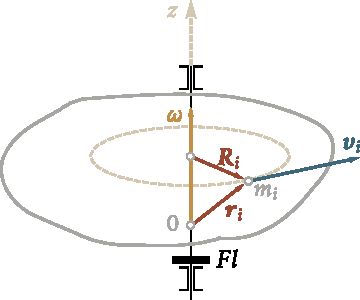
\includegraphics[scale=0.95]{figures/ch_05/fig_5_3.pdf}
			\caption[]{}
			\label{fig:5_3}
		\end{center}
	\end{minipage}
	\hspace{-0.05cm}
	\begin{minipage}[t]{0.5\linewidth}
		\begin{center}
			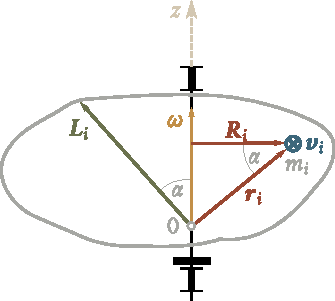
\includegraphics[scale=0.95]{figures/ch_05/fig_5_4.pdf}
			\caption[]{}
			\label{fig:5_4}
		\end{center}
	\end{minipage}
\end{figure}

%A perfectly rigid body can be considered as a system of particles (point particles) with constant distances between them. Equation~\eqref{eq:3_118}, \ie,
Một vật rắn tuyệt đối có thể được xem là một hệ các phần tử (chất điểm) với các khoảng cách giữa chúng là không đổi. Phương trình~\eqref{eq:3_118}, hay
\begin{equation*}
\diff{\vec{L}}{t} = \sum \vec{M}_{\text{ext}}
\end{equation*}

\noindent
%holds for any system of particles, including a rigid body. In the latter case, $\vec{L}$ is the angular momentum of the body. The right-hand side of \eqn{3_118} is the sum of the moments of the external forces acting on the body.
là đúng cho mọi hệ phần tử, bao gồm cả vật rắn. Trong trường hợp này, $\vec{L}$ là momen động lượng của vật. Vế phải của \eqn{3_118} là tổng của tất cả các moment do ngoại lực tác dụng lên vật.

%Let us take point $0$ on the axis of rotation and characterize the position of the particles forming the body with the aid of position vectors $\vec{r}$ drawn from this point (\fig{5_3} depicts the $i$-th particle of mass $m_1$). According to \eqn{3_105}, the angular momentum of the $i$-th particle relative to point $0$ is
Ta hãy lấy điểm $0$ trên trục quay và đặc trưng cho vị trí của các phần tử tạo thành vật bởi các vector bán kính r vẽ từ điểm này (\fig{5_3} mô tả phần tử thứ $i$ có khối lượng $m_i$). Theo như \eqn{3_105}, momen động lượng của hạt thứ $i$ đối với điểm $0$ sẽ là
\begin{equation}\label{eq:5_7}
\vec{L}_i = \vec{r}_i \times m_i\vec{v}_i = m_i\vecprodind{r}{i}{v}{i}.
\end{equation}

\noindent
%The vectors $\vec{r}_i$ and $\vec{v}_i$ are mutually perpendicular for all the particles of the body. Therefore, the magnitude of the vector $\vec{L}_i$ [\eqn{5_7}] is
Các vector $\vec{r}_i$ và $\vec{v}_i$ vuông góc với nhau với tất cả các phần tử của vật. Vì thế độ lớn của vector $\vec{L}_i$ (\eqn{5_7}) là
\begin{equation}\label{eq:5_8}
L_i = m_i r_i v_i = m_i r_i \omega R_i
\end{equation}

\noindent
%\\\\\\\\\\\\\\\\\chờ review////////////////////////
[see \eqn{1_99}]. The direction of the vector $\vec{L}_i$ is shown in \fig{5_4}. It must be noted that the ``length'' of the vector $\vec{L}_i$, according to \eqn{5_8}, is proportional to the velocity of rotation of the body $\vec{\omega}$. The direction of the vector $\vec{L}_i$, however, is independent of $\vec{\omega}$. The vector $\vec{L}_i$ is in a plane passing through the axis of rotation and the particle $m_i$ and is perpendicular to $\vec{r}_i$.
%(xem \eqn{1_99}). Hướng của $\vec{L}_i$ được cho thấy trong \fig{5_4}. Cần phải chú ý rằng "độ dài" của vector $\vec{L}_i$, theo như \eqn{5_8}, tỉ lệ với vận tốc của chuyển động quay của vật $\vec{\omega}$. Tuy nhiên, hướng của vector $\vec{L}_i$ thì không phụ thuộc vào $\vec{\omega}$. Vector $\vec{L}_i$ nằm trong một mặt phẳng đi qua trục quay và phần tử $m_i$, và vuông góc với $\vec{r}_i$.

The projection of the vector $\vec{L}_i$ onto the axis of rotation (the $z$-axis), as can be seen from \fig{5_4}, is [see \eqn{5_8}]
%Dễ dàng khẳng định rằng đối với tất cả các hạt tạo nên vật, góc giữa các vector $\vec{L}_i$ và $\vec{\omega}$ là góc nhọn. Vì vậy, từ \fig{5_4} và \eqn{5_8}, hình chiếu của vector $\vec{L}_i$ lên trục quay (trục $z$) là
\begin{equation}\label{eq:5_9}
L_{zi} = L_i\cos\alpha = m_i r_i \omega R_i \cos\alpha = m_i(r_i\cos\alpha)R_i\omega = m_iR_i^2\omega.
\end{equation}

\begin{figure}[!htb]
	\begin{center}
		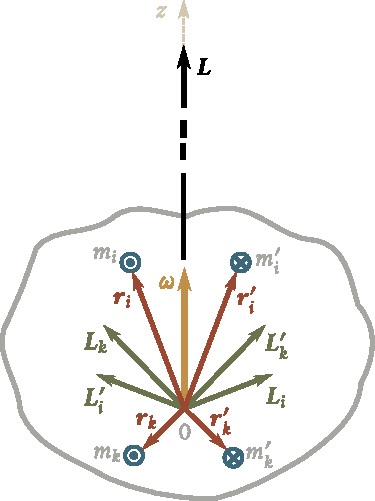
\includegraphics[scale=0.95]{figures/ch_05/fig_5_5.pdf}
		\caption[]{}
		\label{fig:5_5}
	\end{center}
\end{figure}

It is not difficult to see that for a homogeneous\footnote{In mechanics, a body is defined as homogeneous when its density is the same throughout the entire volume (see Sec.~\ref{sec:5_4}).} body which is symmetrical relative to the axis of rotation (for a homogeneous body of revolution), the directions of the total angular momentum (equal to $\sum_i\vec{L}_i$) and of $\vec{\omega}$ along the axis of rotation are the same (\fig{5_5}). Indeed, in this case, the body can be divided into pairs of symmetrically arranged particles of equal mass (two pairs of particles are shown in the figure---$m_i$-$m_i'$ and $m_k$-$m_k'$). The sum of the angular momenta of each pair (in the figure $\vec{L}_i+\vec{L}_i'$ and $\vec{L}_k+\vec{L}_k'$) is directed along the vector $\vec{\omega}$. Hence, the total angular momentum $\vec{L}$ will also coincide in direction with $\vec{\omega}$. The magnitude of the vector $\vec{L}$ in this case equals the sum of the projections of the momenta $\vec{L}_i$ onto the $z$-axis. Taking \eqn{5_9} into account, we get the following expression for the magnitude of the angular momentum of a body:
%Không khó để thấy rằng với một vật đồng chất\footnote{} đối xứng qua trục quay, hướng của momen động lượng toàn phần (bằng $\sum_i\vec{L}_i$) và $\vec{\omega}$ trên trục quay là như nhau (\fig{5_5}). Thật vậy, trong trường hợp này, vật có thể được chia thành các cặp phần tử cùng khối lượng có vị trí đối xứng (hai cặp phần tử như vậy được biểu diễn trong hình vẽ---$m_i$-$m_i'$ và $m_k$-$m_k'$). Tổng của các momen động lượng của mỗi cặp (như trong hình là $\vec{L}_i+\vec{L}_i'$ và $\vec{L}_k+\vec{L}_k'$) có hướng trùng với hướng của $\vec{\omega}$. Do đó, momen động lượng toàn phần $\vec{L}$ cũng sẽ có hướng trùng với hướng của $\vec{\omega}$. Độ lớn của vector $\vec{L}$ lúc này sẽ bằng tổng của các hình chiếu của $\vec{L}_i$ trên trục $z$. Nhắc lại \eqn{5_9}, ta suy ra được biểu thức cho độ lớn của momen động lượng của một vật rắn như sau:
\begin{equation}\label{eq:5_10}
L = \sum_i L_{zi} = \omega \sum_i m_i R_i^2 = I \omega.
\end{equation}

\noindent
The quantity $I$ equal to the sum of the products of the elementary masses and the squares of their distances from a certain axis is called the \textbf{rotational inertia} or the \textbf{moment of inertia of the body} relative to the given axis:
%Đại lượng $I$ bằng tổng của các tích giữa khối lượng nguyên tố và bình phương khoảng cách từ nó đến một trục nhất định được gọi là \textbf{quán tính quay} hoặc \textbf{moment quán tính của vật rắn} đối với trục đó.
\begin{equation}\label{eq:5_11}
I = \sum_i m_i R_i^2.
\end{equation}

\noindent
Summation is performed over all the elementary masses $m_i$ into which the body was mentally divided.
%Phép tính tổng được thực hiện trên tất cả các khối lượng nguyên tố $m_i$ mà vật có thể được chia nhỏ.

\begin{figure}[!htb]
	\begin{minipage}[t]{0.5\linewidth}
		\begin{center}
			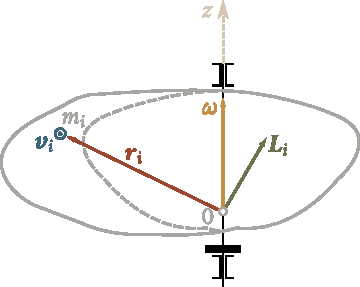
\includegraphics[scale=0.95]{figures/ch_05/fig_5_6.pdf}
			\caption[]{}
			\label{fig:5_6}
		\end{center}
	\end{minipage}
	\hspace{-0.05cm}
	\begin{minipage}[t]{0.5\linewidth}
		\begin{center}
			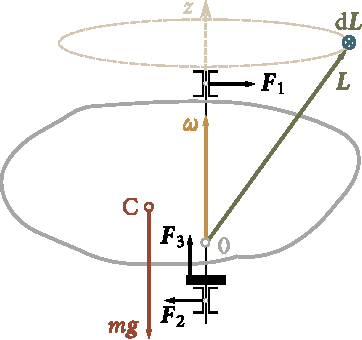
\includegraphics[scale=0.95]{figures/ch_05/fig_5_7.pdf}
			\caption[]{}
			\label{fig:5_7}
		\end{center}
	\end{minipage}
\end{figure}

With a view to the fact that the vectors $\vec{L}$ and $\vec{\omega}$ have identical directions, we can write \eqn{5_10} as follows:
%Để ý rằng các vector $\vec{L}$ và $\vec{\omega}$ có hướng trùng nhau, ta có thể viết lại \eqn{5_10} dưới dạng sau:
\begin{equation}\label{eq:5_12}
\vec{L} = I \vec{\omega}.
\end{equation}

\noindent
%\\\\\\đến đây sự khác biệt không quá đáng kể, nên chú ý bàn luận về phần từ đây trở đi//////
We remind our reader that we have obtained this relation for a homogeneous body rotating about an axis of symmetry. In the general case, as we shall see below, \eqn{5_12} is not obeyed.

For an asymmetrical (or non-homogeneous) body, the angular momentum $\vec{L}$, generally speaking, does not coincide in direction with the vector $\vec{\omega}$. The dash line in \fig{5_6} shows the part of an asymmetrical homogeneous body that is symmetrical relative to the axis of rotation. The total angular momentum of this part, as we have established above, is directed along $\vec{\omega}$. The momentum $\vec{L}_i$ of each particle not belonging to the symmetrical part deviates to the right from the axis of rotation (in a plane figure). Consequently, the total angular momentum of the entire body will also deviate to the right (\fig{5_7}). Upon rotation of the body, the vector $\vec{L}$ rotates together with it, describing a cone. During the time $\deriv{t}$, the vector $\vec{L}$ receives the increment $\deriv{\vec{L}}$, which according to \eqn{3_118} equals
\begin{equation}\label{eq:5_13}
\deriv{\vec{L}} = \left( \sum \vec{M}_{\text{ext}} \right) \, \deriv{t}.
\end{equation}

\noindent
If the vector $\vec{L}$ does not change in magnitude, then the vector $\deriv{\vec{L}}$ is directed beyond the drawing (\fig{5_7}). The vector $\sum\vec{M}_{\text{ext}}$ has the same direction. In the example we are treating, the moments of the external forces include (1) the moment of the force of gravity $m\vec{g}$ directed toward us---we shall call it negative (this force is applied to the centre of mass of the body C), (2) the positive moments of the forces of lateral pressure of the bearings on the axis (the forces $\vec{F}_1$ and $\vec{F}_2$), and (3) the positive moment of the force of pressure of the bearing shoulder on the flange $\vec{F}_3$. We assume that friction forces are absent, otherwise the vector $\vec{L}$ would not be constant in magnitude, and $\deriv{\vec{L}}$ would not be perpendicular to $\vec{L}$.

The angular momentum relative to the axis of rotation [see \eqn{3_108}] for any (homogeneous or non-homogeneous, symmetrical or asymmetrical) body is
\begin{equation}\label{eq:5_14}
L_z = \sum_i L_{zi} = \sum_i m_i R_i^2 \omega = I \omega
\end{equation}

\noindent
(see Eqs.~\eqref{eq:5_9} and \eqref{eq:5_11}]. It must be stressed that unlike \eqn{5_12}, \eqn{5_14} is always correct.

Equation~\eqref{eq:3_119} states that
\begin{equation*}
\diff{L_z}{t} = \sum M_{z,\text{ext}}.
\end{equation*}

\noindent
Introducing into this expression \eqn{5_14} for $L_z$, we get
\begin{equation}\label{eq:5_15}
I \alpha_z = \sum M_{z,\text{ext}}
\end{equation}

\noindent
where $\alpha_z=\dot{\omega}$ is the projection of the angular acceleration onto the $z$-axis (we are considering rotation about a fixed axis, therefore the vector $\vec{\omega}$ can change only in magnitude). Equation~\eqref{eq:5_15} is similar to the equation $m\vec{a}=\vec{F}$. The part of the mass is played by the moment of inertia, that of the linear acceleration by the angular acceleration, and, finally, the part of the resultant force is played by the total moment of the external forces.

In the above example, the moments of all the external forces are perpendicular to the axis of rotation. Hence, their projections onto the $z$-axis equal zero. Accordingly, the angular velocity $\vec{\omega}$ remains constant, which is what should be expected in the absence of friction.

%\\\\\\\\\\\\\\\chờ review/////////////

%We must point out that in the rotation of a homogeneous symmetrical body, forces of lateral pressure of the bearings on the axis (the forces $\vec{F}_1$ and $\vec{F}_2$ in \fig{5_7}) do not appear. In the absence of the force of gravity, we could remove the bearings---the axis would retain its position in space without them. An axis whose position in space remains constant when bodies rotate about it in the absence of external forces is called a \textbf{free axis} of a body.
Chúng ta cần chỉ ra rằng đối với chuyển động quay của một vật đối xứng đồng chất, áp lực ngang của các gối trục tác dụng lên trục (các lực $\vec{F}_1$ và $\vec{F}_2$ trong \fig{5_7}) không tồn tại. Khi không có sự hiện diện của trọng lực, chúng ta có thể loại bỏ các gối trục---trục sẽ giữ nguyên vị trí của nó trong không gian mà không cần chúng. Trục có vị trí không đổi trong không gian khi vật quay quanh nó không dưới tác dụng của ngoại lực được gọi là \textbf{trục tự do} của vật.

%It is possible to prove that for a body of any shape and with an arbitrary arrangement of its mass there are three mutually perpendicular axes passing through the centre of mass of the body that can be free axes. They are called the \textbf{principal axes} of inertia of the body.
Có thể chứng minh được rằng với một vật có hình dạng bất kì và phân bố khối lượng bất kì, sẽ có ba trục cùng vuông góc đi qua khối tâm vật có thể dùng làm các trục tự do. Chúng được gọi là \textbf{các trục quán tính chính} của vật.

\begin{figure}[!htb]
	\begin{minipage}[t]{0.5\linewidth}
		\begin{center}
			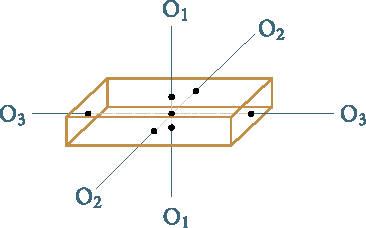
\includegraphics[scale=0.98]{figures/ch_05/fig_5_8.pdf}
			\caption[]{}
			\label{fig:5_8}
		\end{center}
	\end{minipage}
	\hspace{-0.05cm}
	\begin{minipage}[t]{0.5\linewidth}
		\begin{center}
			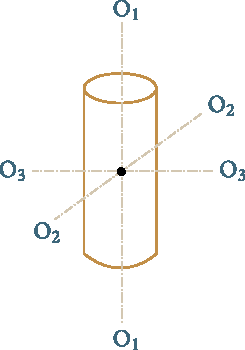
\includegraphics[scale=0.95]{figures/ch_05/fig_5_9.pdf}
			\caption[]{}
			\label{fig:5_9}
		\end{center}
	\end{minipage}
\end{figure}

%In a homogeneous parallelepiped (\fig{5_8}), the principal axes of inertia are obviously the axes O$_1$O$_1$, O$_2$O$_2$, and O$_3$O$_3$ passing through the centres of opposite faces.
Trong một hình hộp đồng chất (\fig{5_8}), dễ thấy rằng các trục quán tính chính là các trục O$_1$O$_1$, O$_2$O$_2$, và O$_3$O$_3$ đi qua tâm của các mặt đối nhau.

%In bodies possessing axial symmetry (for example, in a homogeneous\footnote{It is sufficient that the density of the body in each cross section be a function only of the distance from the axis of symmetry.} cylinder), the axis of symmetry is one of the principal axes of inertia. Any two mutually perpendicular axes in a plane at right angles to the axis of symmetry and passing through the centre of mass of the body can be the other two principal axes (\fig{5_9}). Thus, in such a body only one of the principal axes of inertia is fixed.
Ở những vật có tính đối xứng trục (chẳng hạn như hình trụ đồng chất\footnote{Một cách đầy đủ, khối lượng riêng tại mỗi tiết diện là một hàm của duy nhất một biến là khoảng cách kể từ trục đối xứng} thì trục đối xứng là một trong các trục quán tính chính. Hai trục bất kì vuông góc với nhau trên mặt phẳng vuông góc với trục đối xứng và đi qua khối tâm, có thể được dùng làm hai trục quán tính chính còn lại. Như vậy ở vật đối xứng trục, chỉ có một trục quán tính chính được xác định.

%In a body with central symmetry, \ie, in a sphere whose density depends only on the distance from its centre, any three mutually perpendicular axes passing through the centre of mass are the principal axes of inertia. Consequently, none of the principal axes of inertia is fixed.
Ở vật có đối xứng tâm, như là một quả cầu có khối lượng riêng chỉ phụ thuộc vào khoảng cách tính từ tâm, thì ba trục bất kì vuông góc với nhau và đi qua khối tâm đều có thể là các trục quán tính chính. Do đó không có trục quán tính chính nào là xác định.

%The moments of inertia relative to the principal axes are called the \textbf{principal moments of inertia} of a body. In the general case, these moments differ: $I_1\neq I_2\neq I_3$. For a body with axial symmetry, two of the principal moments of inertia are the same, while the third one, generally speaking, differs from them: $I_1=I_2\neq I_3$. And, finally, for a body with central symmetry, all three principal moments of inertia are the same: $I_1=I_2=I_3$.
Các moment quán tính đối với các trục chính được gọi là \textbf{các moment quán tính chính} của vật. Trong trường hợp tổng quát, các moment này khác nhau: $I_1\neq I_2\neq I_3$. Đối với một vật có đối xứng trục, hai moment quán tính chính có cùng giá trị, trong khi moment thứ ba, nói chung, khác chúng: $I_1=I_2\neq I_3$. Và, cuối cùng, với một vật có đối xứng tâm thì cả ba moment quán tính chính đều bằng nhau: $I_1=I_2=I_3$.

%Not only a homogeneous sphere, but also, for instance, a homogeneous cube has equal values of the principal moments of inertia. In the general case, such equality may be observed for bodies of an absolutely arbitrary shape when their mass is properly distributed. All such bodies are called \textbf{spherical tops}. Their feature is that any axis passing through their centre of mass has the properties of a free axis, and, consequently, none of the principal axes is fixed, as for a sphere. All spherical tops behave the same when they rotate in identical conditions.
Không chỉ với những quả cầu đồng chất mà chẳng hạn như hình lập phương đồng chất cũng có các giá trị moment quán tính chính bằng nhau. Trong trường hợp tổng quát, có thể tìm thấy sự bằng nhau của các moment quán tính chính ở những vật có hình dạng hoàn toàn bất kì nhưng có phân bố khối lượng thích hợp. Những vật như vậy được gọi là các \textbf{con quay cầu}. Đặc điểm của chúng là bất cứ trục nào đi qua khối tâm đều có các tính chất của một trục tự do, và do đó không một trục quán tính chính nào được xác định, giống như một quả cầu. Tất cả các con quay cầu đều thể hiện một cách giống nhau khi được quay trong những điều kiện giống nhau.

%Bodies for which $I_1=I_2\neq I_3$ behave like homogeneous bodies of revolution. They are called \textbf{symmetrical tops}. Finally, bodies for which $I_1=I_2=I_3$ are called \textbf{asymmetrical tops}.
Những vật có $I_1=I_2\neq I_3$ sẽ có biểu hiện giống với của một vật đồng chất quay. Chúng được gọi là \textbf{con quay đối xứng}. Cuối cùng, những vật có $I_1\neq I_2\neq I_3$ được gọi là \textbf{con quay không đối xứng}.

%If a body rotates in conditions when there is no external action, then only rotation about the principal axes corresponding to the maximum and minimum values of the moment of inertia is stable. Rotation about an axis corresponding to an intermediate value of the moment will be unstable. This signifies that the forces appearing upon the slightest deviation of the axis of rotation from this principal axis act in a direction causing the magnitude of this deviation to grow. When the axis of rotation deviates from a stable axis, the forces produced return the body to rotation about the corresponding principal axis.
Nếu một vật quay trong điều kiện không có tác động bên ngoài, thì chỉ có sự quay quanh những trục chính tương ứng với moment quán tính cực đại và cực tiểu là bền. Sự quay quanh một trục tương ứng với một moment có giá trị trung gian sẽ không bền. Điều này có nghĩa khi quay quanh trục không bền, bất kì sự chệch hướng nào dù nhỏ nhất cũng tạo ra một lực tác dụng theo chiều làm tăng độ lớn của sự chệch hướng đó. Ngược lại, khi quay quanh trục bền, lực sinh ra bởi sự chệch hướng sẽ tác dụng theo chiều làm giảm độ lớn của sự chệch hướng, hồi phục lại sự quay quanh trục tương ứng.

\begin{figure}[!htb]
	\begin{center}
		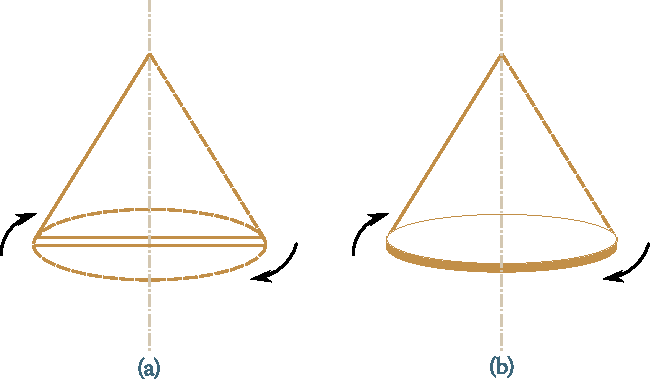
\includegraphics[scale=0.9]{figures/ch_05/fig_5_10.pdf}
		\caption[]{}
		\label{fig:5_10}
	\end{center}
\end{figure}

%We can convince ourselves that what has been said above is true by tossing a body having the shape of a parallelepiped (for example, a match box) and simultaneously bringing it into rotation\footnote{The action of the force of gravity in this case is not significant. It only causes the body to fall in addition to its rotation.}. We shall see that the body when falling can rotate stably about axes passing through the biggest or smallest faces. Attempts to toss the body so that it rotates about an axis passing through the faces of an intermediate size will be unsuccessful.
Chúng ta có thể kiểm chứng xem những điều vừa nói có đúng hay không bằng cách tung lên một vật có dạng hình hộp (chẳng hạn như một hộp diêm) và đồng thời làm cho nó quay\footnote{Tác động của trọng lực trong trường hợp này không đáng kể. Nó chỉ làm cho sự rơi của vật xảy ra cùng với sự quay}. Chúng ta sẽ thấy được rằng khi rơi, vật có thể quay một cách ổn định quanh các trục đi qua các mặt lớn nhất và nhỏ nhất. Các phép thử tung vật sao cho nó quay quanh trục đi qua mặt trung gian đều không thành công.

%If an external force is exerted, for instance, by the string on which a rotating body is suspended, then only rotation about the principal axis corresponding to the maximum value of the moment of inertia will be stable. This is why a thin rod suspended by means of a string fastened to its end when brought into rapid rotation will in the long run rotate about an axis normal to it passing through its centre (\fig{5_10}a). A disk suspended by means of a string fastened to its edge (\fig{5_10}b) behaves in a similar way.
Nếu một ngoại lực được tác dụng, chẳng hạn như từ một sợi dây treo vật đang quay, thì chỉ có sự quay quanh trục chính tương ứng với giá trị lớn nhất của moment quán tính là ổn định. Điều này giải thích vì sao khi một thanh mảnh treo bằng một sợi dây  buộc vào một đầu của nó được quay nhanh, thì sau thời gian dài thanh sẽ quay quanh một trục vuông góc và đi qua tâm của nó. (\fig{5_10}a). Một đĩa treo bằng một sợi dây buộc vào mép đĩa (\fig{5_10}b) cũng biểu hiện tương tự vậy.

%Up to now, we have treated bodies with a constant distribution of their mass. Now let us assume that a rigid body can lose for a certain time its property of a constant arrangement of its parts, and within this time redistribution of the body's mass occurs that results in the moment of inertia changing from $I_1$ to $I_2$. If such a redistribution occurs in conditions when $\sum\vec{M}_{\text{ext}}=0$, then in accordance with the law of conservation of angular momentum the following equation must be observed:
Cho đến giờ, ta đã nói về các vật có phân bố khối lượng đều. Bây giờ hãy giả sử trong một khoảng thời gian nhất định, một vật rắn mất đi tính chất không biến đổi vị trí tương đối giữa các phần của nó, và trong khoảng thời gian này sự phân bố lại của khối lượng của vật dẫn đến việc moment quán tính thay đổi từ $I_1$ đến $I_2$. Nếu sự tái cấu trúc như vậy xảy ra với điều kiện $\sum\vec{M}_{\text{ext}}=0$, thì theo định luật bảo toàn momen động lượng, phương trình sau phải được nghiệm đúng:
\begin{equation}\label{eq:5_16}
I_1\omega_1 = I_2\omega_2
\end{equation}

\noindent
%where $\omega_1$ is the initial, and $\omega_2$ is the final value of the angular velocity of the body. Thus, a change in the moment of inertia leads to a corresponding change in the angular velocity. This explains why a spinning figure skater (or a man on a rotating platform) begins to rotate more slowly when he stretches his arms out, and gains speed when he presses his arms against his body.
trong đó $\omega_1$ là giá trị ban đầu, và $\omega_2$ là giá trị cuối cùng của vận tốc góc của vật. Như vậy sự biến đổi của moment quán tính dẫn đến sự biến đổi tương đương của vận tốc góc. Điều này giải thích vì sao một vận động viên trượt băng nghệ thuật đang quay (hoặc một người đứng trên một cái nền đang quay) sẽ quay chậm hơn khi duỗi cánh tay ra, và tăng tốc khi ép chặt cánh tay vào người.

\section{Moment quán tính}\label{sec:5_4}

%From the definition of the moment of inertia\footnote{In this section, it is expedient to use the symbol $\Delta m_i$ instead of $m_i$ for the elementary mass of a body.} [see \eqn{5_11}]
Từ định nghĩa của moment quán tính\footnote{Trong phần này, sẽ tiện lợi hơn nếu sử dụng $\Delta m_i$ thay vì $m_i$ để kí hiệu cho khối lượng nguyên tố của một vật} (xem \eqn{5_11})
\begin{equation*}
I = \sum_i \Delta m_i R_i^2
\end{equation*}

\noindent
%we can see that it is an additive quantity. This signifies that the moment of inertia of a body equals the sum of the moments of inertia of its parts.
ta có thể thấy rằng nó là một đại lượng cộng tính. Điều này có nghĩa là moment quán tính của vật bằng tổng các moment quán tính của các phần khác của vật.

%We introduced the concept of the moment of inertia when dealing with the rotation of a rigid body. It must be borne in mind, however, that this quantity exists irrespective of rotation. Every body, regardless of whether it is rotating or at rest, has a definite moment of inertia relative to any axis, just like a body has a mass regardless of whether it is moving or at rest.
Chúng ta đưa ra khái niệm moment quán tính khi nghiên cứu sự quay của vật rắn. Nhưng cần để ý rằng đại lượng này tồn tại không chỉ đối với sự quay. Tất cả các vật, không phụ thuộc vào nó đang quay hay đứng yên, đều có một moment quán tính xác định đối với một trục bất kì, tương tự như vật có khối lượng không phụ thuộc vào việc nó đang chuyển động hay đứng yên.

%The distribution of the mass within a body can be characterized with the aid of a quantity called the density. If a body is homogeneous, \ie, its properties are the same at all of its points, then the density is defined as the quantity
Sự phân bố khối lượng trong phạm vi một vật có thể được đặc trưng với sự hỗ trợ của đại lượng tên là khối lượng riêng. Nếu một vật là đồng chất, tức là các tính chất của nó là như nhau tại mọi điểm, thì khối lượng riêng được định nghĩa 
\begin{equation}\label{eq:5_17}
\rho = \frac{m}{V}
\end{equation}

\noindent
%where $m$ and $V$ are the mass and volume of the body, respectively. Thus, the density of a homogeneous body is the mass of a unit of its volume.
trong đó $m$ và $V$ lần lượt là khối lượng và thể tích của vật. Như vậy, khối lượng riêng của một vật đồng chất là khối lượng của một đơn vị thể tích.

%For a body with an unevenly distributed mass, \eqn{5_17} gives the average density. The density at a given point is determined in this case as follows:
Với một vật có phân bố khối lượng không đều, \eqn{5_17} cho khối lượng riêng trung bình. Khối lượng riêng tại một điểm cho trước lúc này được xác định như sau:
\begin{equation}\label{eq:5_18}
\rho = \lim_{\Delta v\to 0} \frac{\Delta m}{\Delta V} = \diff{m}{V}.
\end{equation}

\noindent
%In this expression, $\Delta m$ is the mass contained in the volume $\Delta V$, which in the limit transition contracts to the point at which the density is being determined.
Trong biểu thức này $\Delta m$ là khối lượng chứa trong thể tích $\Delta V$ mà khi chuyển sang giới hạn sẽ thu về một điểm nơi đang xác định khối lượng riêng.

%The limit transition in \eqn{5_18} must not be understood in the sense that $\Delta V$ contracts literally to a point. If such a meaning is implied, we would get a greatly differing result for two virtually coinciding points, one of which is at the nucleus of an atom, while the other is at a space between nuclei (the density for the first point would be enormous, and for the second one it would be zero). Therefore, $\Delta V$ should be diminished until we get an infinitely small volume from the physical viewpoint. We understand this to mean such a volume which on the one hand is small enough for the macroscopic (\ie, belonging to a great complex of atoms) properties within its limits to be considered identical, and on the other hand is sufficiently great to prevent discreteness (discontinuity) of the substance from manifesting itself.
Không được hiểu sự chuyển qua giới hạn trong \eqn{5_18} theo đúng nghĩa đen là $\Delta V$ tập trung về một điểm. Nếu thực sự áp dụng ý nghĩa đó, ta sẽ tính được hai kết quả vô cùng chênh lệch tại hai điểm gần như trùng nhau, một điểm là tại hạt nhân của nguyên tử, điểm còn lại là khoảng không gian ở giữa các nguyên tử (khối lượng riêng tại điểm thứ nhất sẽ khổng lồ, còn tại điểm thứ hai thì bằng không). Do đó, $\Delta V$ sẽ chỉ co nhỏ lại cho đến khi ta thu được một thể tích vô cùng bé xét về phương diện vật lý, nghĩa là một mặt đủ nhỏ để có thể coi các tính chất vĩ mô (của một tập hợp lớn các nguyên tử chẳng hạn) trong phạm vi đó là đồng nhất, mặt khác đủ lớn để sự gián đoạn (sự rời rạc) của vật chưa đáng kể.

%By \eqn{5_18}, the elementary mass $\Delta m_i$ equals the product of the density of a body $\rho_i$ at a given point and the corresponding elementary volume $\Delta V_i$:
Theo \eqn{5_18}, khối lượng nguyên tố $\Delta m_i$ bằng tích của khối lượng riêng của vật $\rho$ tại điểm đang xét nhân cho thể tích nguyên tố tương ứng.
\begin{equation*}
\Delta m_i = \rho_i \Delta V_i.
\end{equation*}

\noindent
%Consequently, the moment of inertia can be written in the form
Do đó có thể viết moment quán tính dưới dạng
\begin{equation}\label{eq:5_19}
I = \sum_i \rho_i R_i^2 \Delta V_i.
\end{equation}

\noindent
%If the density of a body is constant, it can be put outside the sum:
Nếu khối lượng riêng của vật không đổi, nó có thể đưa ra ngoài dấu tổng:
\begin{equation}\label{eq:5_20}
I = \rho \sum_i R_i^2 \Delta V_i.
\end{equation}

%Equations~\eqref{eq:5_19} and \eqref{eq:5_20} are approximate. Their accuracy grows with diminishing elementary volumes $\Delta V_i$ and the elementary masses $\Delta m_i$ corresponding to them. Hence, the task of finding the moments of inertia consists in integration:
Các phương trình~\eqref{eq:5_19} và \eqref{eq:5_20} là các phương trình gần đúng. Độ chính xác của chúng càng tăng khi thể tích nguyên tố $\Delta V_i$ và khối lượng nguyên tố tương ứng càng nhỏ. Do đó, bài toán tìm các moment quán tính dẫn tới phép tính tích phân:
\begin{equation}\label{eq:5_21}
I = \int R^2\, \deriv{m} = \int \rho R^2\, \deriv{V}.
\end{equation}

\noindent
%The integrals in \eqn{5_21} are taken over the entire volume of the body. The quantities $\rho$ and $R$ in these integrals are position functions, \ie, for example, functions of the Cartesian coordinates $x$, $y$, and $z$.
Các tích phân trong \eqn{5_21} được tính theo toàn bộ thể tích của vật. Các đại lượng $\rho$ và $R$ trong các tích phân này là các hàm vị trí, tức là một hàm theo các tọa độ Descartes $x$, $y$, và $z$ chẳng hạn.

%As an example, let us find the moment of inertia of a homogeneous disk relative to an axis perpendicular to the plane of the disk and passing through its centre (\fig{5_11}). Let us divide the disk into annular layers of thickness $\deriv{R}$. All the points of one layer will be at the same distance $R$ from the axis. The volume of such a layer is
Để ví dụ, ta hãy tính moment quán tính của một cái đĩa đồng chất đối với một trục vuông góc với mặt phẳng của đĩa và đi qua tâm của nó (\fig{5_11}). Ta chia đĩa thành các lớp hình vành khăn có độ dày $\deriv{R}$. Mọi điểm trên một lớp sẽ có cùng khoảng cách $R$ tính từ trục. Thể tích của một lớp như vậy bằng
\begin{equation*}
\deriv{V} = 2\pi bR\,\deriv{R}
\end{equation*}

\noindent
%where $b$ is the thickness of the disk.
trong đó $b$ là độ dày của đĩa

%Since the disk is homogeneous, its density at all its points is the same, and $\rho$ in \eqn{5_21} can be put outside the integral:
Do đĩa đồng chất, khối lượng riêng của nó tại mọi điểm đều như nhau, và $\rho$ trong \eqn{5_21} có thể được đưa ra ngoài dấu tích phân:
\begin{equation*}
I = \rho \int R^2\,\deriv{V} = \rho \int_0^{R_0} R^2 2\pi bR\,\deriv{R}
\end{equation*}

\noindent
%where $R_0$ is the radius of the disk. Let us put the constant factor $2\pi b$ outside the integral:
trong đó $R_0$ là bán kính của đĩa. Ta hãy đưa hệ số hằng $2\pi b$ ra ngoài dấu tích phân:
\begin{equation*}
I = 2\pi b\rho \int_0^{R_0} R^3\,\deriv{R} = 2\pi b\rho\frac{R^4_0}{4}.
\end{equation*}

\noindent
%Finally, introducing the mass of the disk $m$ equal to the product of the density $\rho$ and the volume of the disk $b\pi R^2_0$, we get
Cuối cùng, đặt khối lượng $m$ của đĩa bằng tích của khối lượng riêng nhân thể tích của đĩa $b\pi R_0^2$, ta thu được
\begin{equation}\label{eq:5_22}
I = \frac{mR_0^2}{2}.
\end{equation}

\begin{figure}[!htb]
	\begin{center}
		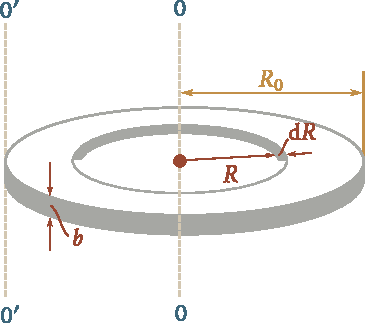
\includegraphics[scale=0.95]{figures/ch_05/fig_5_11.pdf}
		\caption[]{}
		\label{fig:5_11}
	\end{center}
\end{figure}

%The finding of the moment of inertia in the above example was simplified quite considerably owing to the fact that the body was homogeneous and symmetrical, and we sought the moment of inertia relative to an axis of symmetry. If we wanted to find the moment of inertia of the disk relative, for example, to the axis $0'0'$ perpendicular to the disk and passing through its edge (see \fig{5_11}), the calculations would evidently be much more complicated. The finding of the moment of inertia is considerably simplified in such cases if we use the Steiner or parallel axis theorem, which is formulated as follows: \textit{the moment of inertia $I$ relative to an arbitrary axis equals the moment of inertia $I_{\text{C}}$ relative to an axis parallel to the given one and passing through the body's centre of mass plus the product of the body's mass $m$ and the square of the distance $b$ between the axes}:
Việc tìm moment quán tính trong ví dụ vừa xét đã được đơn giản hóa rất nhiều vì vật đồng chất và đối xứng, mà ta lại đang tìm moment quán tính đối với trục đối xứng. Nếu ta muốn tìm moment quán tính của đĩa đối với, chẳng hạn như, trục $0'0'$ vuông góc với đĩa và đi qua mép của nó (xem \fig{5_11}), thì việc tính toán rõ ràng là phức tạp hơn nhiều. Việc tìm moment quán tính của những trường hợp tương tự vậy sẽ trở nên đơn giản hơn nhiều nếu dùng định lý Steiner hay định lý trục quay song song, được phát biểu như sau: \textit{moment quán tính $I$ đối với một trục bất kì bằng tổng của moment quán tính $I_{\text{C}}$ đối với một trục đi qua khối tâm, song song với trục ban đầu và tích của khối lượng vật $m$ và bình phương khoảng cách $b$ giữa hai trục}
\begin{equation}\label{eq:5_23}
I = I_{\text{C}}+ mb^2.
\end{equation}

%According to the parallel axis theorem, the moment of inertia of the disk relative to the axis $0'0'$ equals the moment of inertia relative to the axis passing through the centre of the disk, which we have found [\eqn{5_22}] plus $mR_0^2$ (the distance between the axes $0'0'$ and $00$ equals the radius of the disk $R_0$):
Theo định lý trục quay song song, moment quán tính của đĩa đối với trục $0'0'$ bằng moment quán tính đối với trục đi qua tâm của đĩa mà ta đã tìm ra ở \eqn{5_22} cộng với $mR_0^2$ (khoảng cách giữa hai trục $0'0'$ và $00$ bằng bán kính $R_0$ của đĩa)
\begin{equation*}
I = \frac{mR^2_0}{2} + mR_0^2 = \frac{3}{2}mR_0^2.
\end{equation*}

%Thus, the parallel axis theorem in essence reduces the calculation of the moment of inertia relative to an arbitrary axis to the calculation of the moment of inertia relative to an axis passing through the centre of mass of the body.
Như vậy, điều cốt lõi của định lý trục quay song song là rút gọn từ bài toán tìm moment quán tính đối với trục bất kì về bài toán tìm moment quán tính đối với trục đi qua khối tâm.

\begin{figure}[!htb]
	\begin{center}
		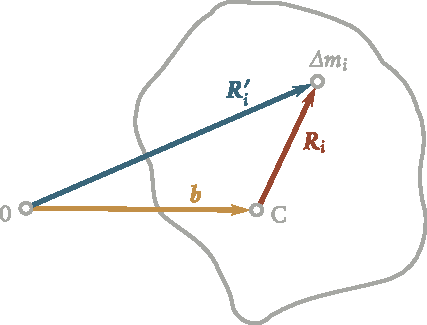
\includegraphics[scale=0.93]{figures/ch_05/fig_5_12.pdf}
		\caption[]{}
		\label{fig:5_12}
	\end{center}
\end{figure}

%To prove the parallel axis theorem, let us consider axis C passing through the centre of mass of a body and axis $0$ parallel to it and at a distance $b$ from axis C (\fig{5_12}, both axes are perpendicular to the plane of the drawing). Let $\vec{R}_i$ be a vector perpendicular to axis C and drawn from the axis to the elementary mass $\Delta m_i$ and $\Delta\vec{R}_i$ be a similar vector drawn from axis $0$. We shall also introduce the vector $\vec{b}$ perpendicular to the axes and connecting the corresponding points of axes $0$ and C. For any pair of points opposite each other, this vector has the same value (equal to the distance $b$ between the axes) and the same direction. The following relation holds between the vectors listed above:
Để chứng minh định lý trục quay song song, ta xét một trục C đi qua khối tâm của vật và một trục $0$ song song, đứng cách trục C một khoảng $b$ (\fig{5_12}, cả hai trục đều vuông góc với mặt phẳng hình vẽ). Đặt $\vec{R}_i$ là vector vuông góc với trục C và hướng từ trục này đến khối lượng nguyên tố $\Delta m_i$, còn $\Delta R_i$ là vector tương tự hướng từ trục $0$. Ta cũng đưa vào vector $\vec{b}$ vuông góc với các trục và nối các điểm tương ứng của các trục $0$ và C. Với mọi cặp điểm bất kì nằm đối diện nhau vector này có cùng độ lớn (bằng khoảng cách b giữa các trục) và cùng hướng. Giữa các vector trên có hệ thức:
\begin{equation*}
\vec{R}_i' = \vec{b} + \vec{R}_i.
\end{equation*}

%The square of the distance to the elementary mass $\Delta m_i$ from axis C is $R_i^2=\vec{R}^2$, and from axis $0$ is
Bình phương khoảng cách từ trục C đến khối lượng nguyên tố $\Delta m_i$ bằng $R_i^2=\vec{R}^2$, còn từ trục $0$ tới $\Delta m_i$ bằng
\begin{equation*}
R_i'^2 = (\vec{b} + \vec{R}_i)^2 = b^2 + 2\vecdot{b}{R}_i + R_i^2.
\end{equation*}

\noindent
%With a view to the above expression, the moment of inertia of the body relative to axis $0$ can be written in the form
Nếu chú ý tới biểu thức trên, có thể biểu diễn moment quán tính của vật đối với trục $0$ dưới dạng
\begin{equation}\label{eq:5_24}
I = \sum_i \Delta m_i R_i'^2 = b^2 \sum_i \Delta m_i + 2\vec{b} \sum_i \Delta m_i \vec{R}_i + \sum_i \Delta m_i R_i^2
\end{equation}

\noindent
%(we have put the constant factors outside the sum). The last term in this expression is the moment of inertia of the body relative to axis C. Let us designate it $I_{\text{C}}$. The sum of the elementary masses gives the mass of the body $m$. The sum $\sum_i\Delta m_i\vec{R}_i$ equals the product of the mass of the body and the vector $\vec{R}$ drawn from axis C to the centre of mass of the body. Since the centre of mass is on axis C, this vector $\vec{R}$ and, consequently, the second term in \eqn{5_24} vanish. We thus arrive at the conclusion that
(ta có thể đưa các hệ số hằng ra ngoài dấu tổng). Số hạng cuối cùng của biểu thức này là moment quán tính của vật đối với trục C. Ta kí hiệu nó là $I_{\text{C}}$. Tổng các khối lượng nguyên tố cho khối lượng $m$ của vật. Tổng $\sum_i\Delta m_i\vec{R}_i$ bằng tích của khối lượng vật và vector $\vec{R}$ vẽ từ trục C đến khối tâm vật. Vì tâm quán tính nằm trên trục C nên vector $\vec{R}$, và do đó, cả số hạng thứ hai trong \eqn{5_24} đều bằng không. Như vậy ta đi tới kết luận là
\begin{equation*}
I = mb^2 + I_{\text{C}}
\end{equation*}

\noindent
%Q.E.D [see \eqn{5_23}].
đó là điều phải chứng minh (xem \eqn{5_23})

%In concluding, we shall give the values of the moments of inertia for selected bodies (the latter are assumed to be homogeneous, $m$ is the mass of the body).
Để kết thúc phần này, ta hãy đưa ra các giá trị của các moment quán tính đối với một vài vật (các vật được giả thiết là đồng chất, $m$ là khối lượng của vật).
\begin{enumerate}[1.]
	\item Vật là một thanh dài mảnh với tiết diện có hình dạng bất kì. Kích thước tiết diện cực đại $b$ của thanh rất bé so với độ dài $l$ ($b \ll l$). Moment quán tính đối với trục vuông góc với thanh và đi qua trung điểm của nó (\fig{5_13}) bằng %The body is a thin long rod with a cross section of any shape. The maximum cross-sectional dimension $b$ of the rod is many times smaller than its length $l$ ($b\sim l$). The moment of inertia relative to an axis perpendicular to the rod and passing through its middle (\fig{5_13}) is
	\begin{equation}\label{eq:5_25}
	I = \frac{1}{12}ml^2.
	\end{equation}
	
	\begin{figure}[!htb]
	\begin{minipage}[t]{0.5\linewidth}
		\begin{center}
			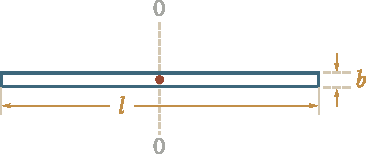
\includegraphics[scale=0.95]{figures/ch_05/fig_5_13.pdf}
			\caption[]{}
			\label{fig:5_13}
		\end{center}
	\end{minipage}
	\hspace{-0.05cm}
	\begin{minipage}[t]{0.5\linewidth}
		\begin{center}
			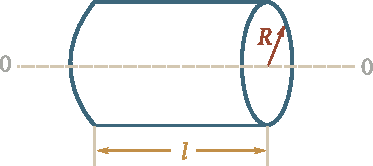
\includegraphics[scale=0.9]{figures/ch_05/fig_5_14.pdf}
			\caption[]{}
			\label{fig:5_14}
		\end{center}
	\end{minipage}
\end{figure}

	\item Đối với một đĩa hoặc một hình trụ với một tỷ số bất kì giữa $R$ và $l$ (\fig{5_14}), moment quán tính đối với trục trùng với trục hình học của trụ bằng  %For a disk or cylinder with any ratio of $R$ to $l$ (\fig{5_14}), the moment of inertia relative to an axis coinciding with the geometrical axis of the cylinder is
	\begin{equation}\label{eq:5_26}
	I = \frac{1}{2}mR^2.
	\end{equation}
	
	\begin{figure}[!htb]
	    \begin{center}
		    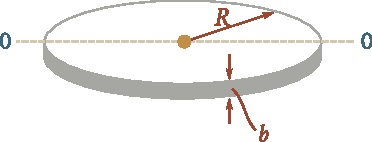
\includegraphics[scale=0.95]{figures/ch_05/fig_5_15.pdf}
		    \caption[]{}
		    \label{fig:5_15}
	    \end{center}
    \end{figure}

	\item Vật là một đĩa mỏng. Độ dày $b$ của đĩa rất nhỏ so với bán kính $R$ của đĩa ($b \ll R$). Moment quán tính đối với trục trùng với một đường kính bất kì của đĩa (\fig{5_15}) là %The body is a thin disk. The thickness of the disk $b$ is many times smaller than the radius of the disk $R$ ($b\sim R$). The moment of inertia relative to an axis coinciding with the diameter of the disk (\fig{5_15}) is
	\begin{equation}\label{eq:5_27}
		I = \frac{1}{4}mR^2.
	\end{equation}

	\item Moment quán tính của một quả cầu bán kính $R$ đối với một trục bất kì đi qua tâm của nó bằng %The moment of inertia of a sphere of radius $R$  relative to an axis passing through its centre is
	\begin{equation}\label{eq:5_28}
		I = \frac{2}{5}mR^2.
	\end{equation}
\end{enumerate}

\section{Khái niệm về tensor quán tính}\label{sec:5_5}

%We established in Sec.~\ref{sec:5_3} that for a homogeneous body rotating about an axis of symmetry, the relation between the vectors $\vec{L}$ and $\vec{\omega}$ has a very simple form [\eqn{5_12}]
Ta đã chứng minh trong Sec.~\ref{sec:5_3} rằng với một vật đồng chất quay quanh một trục đối xứng, liên hệ giữa các vector $\vec{L}$ và $\vec{\omega}$ có dạng rất đơn giản [\eqn{5_12}]
\begin{equation*}
\vec{L} = I\vec{\omega}
\end{equation*}

\noindent
%or
hoặc
\begin{equation}\label{eq:5_29}
L_x = I\omega_x,\quad L_y = I\omega_y,\quad L_z = I\omega_z.
\end{equation}

\noindent
%The explanation is that for such a body the vectors $\vec{L}$ and $\vec{\omega}$ are collinear. In the general case, however, the vectors $\vec{L}$ and $\vec{\omega}$ make an angle differing from zero (see \fig{5_7}), so that the relation between them cannot be expressed by \eqn{5_12}.
Điều này được giải thích là đối với một vật như thế, các vector $\vec{L}$ và $\vec{\omega}$ đều đồng phương. Tuy nhiên trong trường hợp tổng quát, các vector $\vec{L}$ và $\vec{\omega}$ hợp với nhau một góc khác không (xem \fig{5_7}), cho nên liên hệ giữa chúng không thể được biểu diễn bởi \eqn{5_12} nữa.

%Let us try to find a way of relating the vectors $\vec{L}$ and $\vec{\omega}$ analytically in the most general case. We shall proceed from the fact that the magnitudes of $\vec{L}$ and $\vec{\omega}$ are proportional to each other. Indeed, according to \eqn{5_8}, the magnitudes of the elementary vectors $\vec{L}_i$ are proportional to the magnitude of $\vec{\omega}$. Hence, the magnitude of the sum of these vectors is also proportional to $\vec{\omega}$. It is easy to understand that such proportionality is obtained when each component of the vector $\vec{L}$ depends linearly on the components of the vector $\vec{\omega}$:
Ta hãy thử tìm xem có thể liên hệ bằng giải tích các vector $\vec{L}$ và $\vec{\omega}$ trong trường hợp tổng quát nhất. Ta sẽ xuất phát từ việc độ lớn của $\vec{L}$ và $\vec{\omega}$ tỉ lệ với nhau. Thật vậy, theo \eqn{5_8}, độ lớn của vector nguyên tố $\vec{L}_i$ tỉ lệ với độ lớn của $\vec{\omega}$, cho nên tổng của độ lớn các vector này cũng sẽ tỉ lệ với $\vec{\omega}$. Dễ dàng hiểu được rằng sự tỉ lệ đó thu được trong trường hợp nếu mỗi thành phần của vector $\vec{L}$ phụ thuộc một các tuyến tính vào các thành phần của vector $\vec{\omega}$:
\begin{align}
L_x &= I_{xx}\omega_x + I_{xy}\omega_y + I_{xz}\omega_z\nonumber\\
L_y &= I_{yx}\omega_x + I_{yy}\omega_y + I_{yz}\omega_z\label{eq:5_30}\\
L_z &= I_{zx}\omega_x + I_{zy}\omega_y + I_{zz}\omega_z.\nonumber
\end{align}

\noindent
%Here the quantities $I_{xx}, I_{xy}$, etc. are proportionality constants having the dimension of the moment of inertia [compare with \eqn{5_29}]. When $\vec{\omega}$ increases a certain number of times, each of the components $\omega_x, \omega_y, \omega_z$, and accordingly each of the components $L_x, L_y, L_z$ grows the same number of times, as, consequently, does the vector $\vec{L}$ itself.
Ở đây các đại lượng $I_{xx}, I_{xy}$, v.v... là các hệ số tỉ lệ có thứ nguyên của moment quán tính (so sánh với \eqn{5_29}). Khi $\vec{\omega}$ tăng một số lần nào đó, mỗi thành phần $\omega_x, \omega_y, \omega_z$, và tương ứng là các thành phần $L_x, L_y, L_z$ cũng sẽ tăng chừng ấy lần, nghĩa là chính vector $\vec{L}$ cũng sẽ tăng như vậy.

%The mutual orientation of the vectors $\vec{L}$ and $\vec{\omega}$ is determined by the values of the proportionality constants. Assume, for example, that $I_{xx}=I_{yy}=I_{zz}$, and the remaining constants equal zero. In this case, Eqs.~\eqref{eq:5_30} transform into Eqs.~\eqref{eq:5_29}, \ie, the vectors $\vec{L}$ and $\vec{\omega}$ will be collinear. Now let us assume that the vector $\vec{\omega}$ is directed along the $z$-axis, and the constants $I_{xz}, I_{yz}, I_{zz}$ differ from zero. In this case $\omega_z=\omega, \omega_x=\omega_y=0$. Substitution of these values in Eqs.~\eqref{eq:5_30} yields
Sự định hướng tương hỗ của các vector $\vec{L}$ và $\vec{\omega}$ được xác định bằng các giá trị của các hệ số tỉ lệ. Chẳng hạn, giả sử $I_{xx}=I_{yy}=I_{zz}$ và các hệ số hằng còn lại đều bằng không. Khi đó, \eqref{eq:5_30} chuyển thành \eqref{eq:5_29}, tức là các vector $\vec{M}$ và $\vec{\omega}$ đồng phương. Bây giờ ta giả sử rằng vector $\vec{\omega}$ hướng dọc theo trục $z$, và các hệ số $I_{xz}, I_{yz}, I_{zz}$ khác không. Trong trường hợp này $\omega_z=\omega, \omega_x=\omega_y=0$. Thế các giá trị này vào \eqref{eq:5_30} cho ra
\begin{equation*}
L_x = I_{xz}\omega\neq 0,\quad L_y = I_{yz}\omega\neq 0,\quad L_z = I_{zz}\omega\neq 0.
\end{equation*}

\noindent
%All three components of the vector $\vec{L}$ differ from zero. Hence, the vector $\vec{L}$ makes a certain angle with the vector $\vec{\omega}$ directed along the $z$-axis.
Cả ba thành phần của vector $\vec{L}$ đều khác không, do đó vector $\vec{L}$ tạo một góc nhất định với vector $\vec{\omega}$ hướng theo trục $z$.

%It follows from the above that in the most general case the relation between the angular momentum and the angular velocity of a body can be expressed with the aid of Eqs.~\eqref{eq:5_30}. Similar equations can be written for any vectors $\vec{a}$ and $\vec{b}$ whose magnitudes are proportional to each other:
Từ điều trên suy ra rằng trong trường hợp tổng quát nhất, sự liên hệ giữa moment động lượng và vận tốc góc của vật có thể được biểu diễn bằng các công thức \eqref{eq:5_30}. Các công thức tương tự có thể được viết với mọi vector $\vec{a}$ và $\vec{b}$ bất kì có các module tỉ lệ với nhau:
\begin{align}
	b_x &= T_{xx} a_x + T_{xy} a_y + T_{xz} a_z\nonumber\\
	b_y &= T_{yx} a_x + T_{yy} a_y + T_{yz} a_z \label{eq:5_31} \\
	b_z &= T_{zx} a_x + T_{zy} a_y + T_{zz} a_z.\nonumber
\end{align}

\noindent
%These three equations can be written compactly in the form of a single expression:
Ba phương trình này có thể được viết rút gọn dưới dạng một biểu thức:
\vspace{-12pt}
\begin{equation}\label{eq:5_32}
b_i = \sum_{k=x,y,z} T_{ik} a_k.
\end{equation}

\noindent
%Assuming that $i=x$ and performing summation with the subscript $k$ sequentially having the values $x,y,z$, we get the first of the equations~\eqref{eq:5_31}, assuming that $i=y$, we get the second equation, etc.
Đặt $i=x$ và thực hiện phép lấy tổng, trong đó chỉ số $k$ lần lượt lấy các giá trị $x,y,z$, ta được phương trình thứ nhất trong các phương trình~\eqref{eq:5_31}. Đặt $i=y$, ta được công thức thứ hai, v.v...

%The combination of the nine quantities $T_{xx}, T_{xy}, \ldots, T_{zz}$ is called a \textbf{tensor of rank two}\footnote{A tensor of rank two is defined as a combination of the nine quantities $T_{xx}, T_{xy}, \ldots, T_{zz}$ that transform according to definite rules upon rotations of the coordinate axes.}, and the operation expressed by Eqs.~\eqref{eq:5_31} is called multiplication of the vector $\vec{a}$ by the tensor $T$. Such multiplication produces a new vector $\vec{b}$.
Tập hợp chín đại lượng $T_{xx}, T_{xy}, \ldots, T_{zz}$ được gọi là một \textbf{tensor hạng hai}\footnote{Tensor hạng hai được định nghĩa là tập hợp chín đại lượng $T_{xx}, T_{xy}, \ldots, T_{zz}$ biến đổi theo các quy tắc nhất định khi quay quanh các trục tọa độ.}, còn phép toán biểu thị bởi \eqref{eq:5_31} được gọi là phép nhân vector $\vec{a}$ với tensor $T$. Phép nhân đó tạo ra một vector mới $\vec{b}$.

%It is customary practice to write a tensor in the form of a square table\footnote{More commonly known as matrix form --Ed.}:
Tensor thường được viết dưới dạng một bảng hình vuông\footnote{Cái tên phổ biến hơn là ma trận}:
\begin{equation}\label{eq:5_33}
	T = \begin{pmatrix}
		T_{xx}&T_{xy}&T_{xz}\\
		T_{yx}&T_{yy}&T_{yz}\\
		T_{zx}&T_{zy}&T_{zz}
		\end{pmatrix}
\end{equation}

\noindent
%(we can write the subscripts $1, 2, 3$ instead of $x, y, z$). The quantities $T_{xx}, T_{xy}, \ldots$ are defined as the components of the tensor. The components $T_{xx}, T_{yy}, T_{zz}$ along the diagonal of matrix~\eqref{eq:5_33} are called diagonal ones. The values of the components depend on the choice of the coordinate axes onto which the vectors $\vec{a}$ and $\vec{b}$ are projected (the components of these vectors also depend on the choice of the axes).
(ta có thể viết các chỉ số $1, 2, 3$ thay vì $x, y, z$).  Các đại lượng $T_{xx}, T_{xy}, \ldots$ được gọi là các thành phần của tensor. Các thành phần $T_{xx}, T_{yy}, T_{zz}$ nằm trên đường chéo của ma trận~\eqref{eq:5_33} được gọi là các thành phần chéo. Các giá trị của các thành phần phụ thuộc vào việc lựa chọn các trục tọa độ và trên đó người ta chiếu các vector$\vec{a}$ và $\vec{b}$ (cả các thành phần của các vector thành phần này cũng phụ thuộc vào việc chọn trục).

%A comparison of Eqs.~\eqref{eq:5_30} and \eqref{eq:5_31} shows that the constants in Eqs.\eqref{eq:5_30} are the components of a tensor of rank two:
So sánh \eqref{eq:5_30} và \eqref{eq:5_31} cho thấy các hệ số hằng trong \eqref{eq:5_30} chính là các thành phần của một tensor hạng hai:
\begin{equation}\label{eq:5_34}
	I = \begin{pmatrix}
		I_{xx}&I_{xy}&I_{xz}\\
		I_{yx}&I_{yy}&I_{yz}\\
		I_{zx}&I_{zy}&I_{zz}
	\end{pmatrix}.
\end{equation}

\noindent
%It is called the \textbf{inertia tensor} of a body. This tensor characterizes the inertia properties of a body in rotation.
Người ta gọi đó là \textbf{tensor quán tính} của một vật. Tensor này đặc trưng cho mức quán tính của vật trong chuyển động quay.

\begin{figure}[!htb]
	\begin{center}
		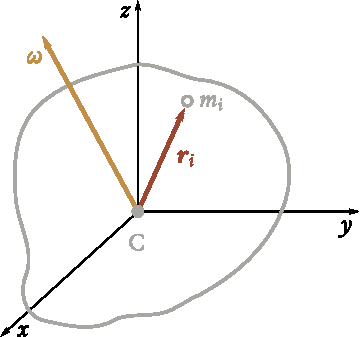
\includegraphics[scale=1.0]{figures/ch_05/fig_5_16.pdf}
		\caption[]{}
		\label{fig:5_16}
	\end{center}
\end{figure}

%To find the values of the components of the inertia tensor, we shall proceed from the definition of the angular momentum of a body:
Để tìm các giá trị của các thành phần của tensor quán tính, ta hãy xuất phát từ định nghĩa của moment động lượng của một vật:
\begin{equation}\label{eq:5_35}
\vec{L} = \sum_i m_i [\vecprodind{r}{i}{v}{i}]
\end{equation}

\noindent
%[see \eqn{5_7}]. We shall plot the vectors $\vec{r}_i$ from the centre of mass of a body (\fig{5_16}). Let us substitute the vector product $\vecprod{\omega}{r}_i$ for the velocity $\vec{v}_i$ in \eqn{5_35} [see \eqn{1_100}]. We get
[xem \eqn{5_7}]. Ta sẽ đặt các vector $\vec{r}_i$ từ khối tâm của vật (\fig{5_16}). Hãy thay vận tốc $\vec{v}_i$ trong \eqn{5_35} [xem \eqn{1_100}]. Kết quả là ta thu được:
\begin{equation*}
\vec{L} = \sum_i m_i [\vec{r}_i \times (\vec{\omega} \times \vec{r}_i)].
\end{equation*}

\noindent
%We shall now use \eqn{1_35}:
Giờ ta sẽ dùng "bac-cab" \eqn{1_35}:
\begin{equation}\label{eq:5_36}
\vec{L} = \sum_i m_i [\vec{\omega}(\vec{r}_i\boldsymbol{\cdot}\vec{r}_i) - \vec{r}_i(\vec{r}_i\boldsymbol{\cdot}\vec{\omega})].
\end{equation}

\noindent
%We remind our reader that summation is conducted of all the elementary masses into which we have mentally divided the body.
Ta nhớ rằng phép lấy tổng được thực hiện theo tất cả các khối lượng nguyên tố mà vật được chia trong tưởng tượng.

%Let us associate a Cartesian system of coordinates with the body\footnote{It must be stressed that the axes of this system are rigidly associated with the body and rotate together with it.} (see \fig{5_16}) and write the scalar products figuring in \eqn{5_16} through the components of the vectors $\vec{\omega}$ and $\vec{r}_i$ along the axes of this system [see~\eqn{1_23}]. We place the origin of coordinates at the centre of mass of the body C (it must be remembered that we plotted the vectors $\vec{r}_i$ from this point). Taking into account that $r_{xi}=x_i, r_{yi}=y_i, r_{zi}=z_i$, we get
Hãy gắn hệ tọa độ Decartes với vật\footnote{Cần nhấn mạnh rằng các trục của hệ này gắn với vật và xoay cùng với nó.} (xem \fig{5_16}) và viết các tích vô hướng có mặt trong \eqn{5_16} qua các thành phần của các vector $\vec{\omega}$ và $\vec{r}_i$ theo các trục của hệ này (xem~\eqn{1_23}). Ta đặt gốc tọa độ tại khối tâm C của vật (nhớ rằng ta đã đặt các vector $\vec{r}_i$ từ điểm này). Nếu chú ý rằng $r_{xi}=x_i, r_{yi}=y_i, r_{zi}=z_i$, ta thu được:
\begin{equation}\label{eq:5_37}
\vec{L} = \sum_i m_i [\vec{\omega}(x_i^2+y_i^2+z_i^2) - \vec{r}_i(x_i\omega_x+y_i\omega_y+z_i\omega_z)].
\end{equation}

\noindent
%Let us find the projection of this vector onto the $x$-axis:
Hãy tìm hình chiếu của vector này lên trục $x$:
\begin{align}
L_x &= \sum_i m_i [\omega_x(x_i^2+y_i^2+z_i^2) - x_i(x_i\omega_x+y_i\omega_y+z_i\omega_z)] \nonumber\\
&= \omega_x\sum_i m_i(y_i^2+z_i^2) - \omega_y\sum_i m_i x_i y_i - \omega_z\sum_i m_i x_i z_i.\label{eq:5_38}
\end{align}

\noindent
%In a similar way, we find the projections of the vector $\vec{L}$ onto the axes $y$ and $z$:
Một cách tương tự, người ta tìm được các hình chiếu của vector $\vec{L}$ lên trục $y$ và $z$:
\begin{align}
L_y &= -\omega_x\sum_i m_i y_i x_i + \omega_y\sum_i m_i (x_i^2+z_i^2) - \omega_z\sum_i m_i y_i z_i \label{eq:5_39}\\
L_z &= -\omega_x\sum_i m_i z_i x_i - \omega_y\sum_i m_i z_i y_i + \omega_z\sum_i m_i (x_i^2+y_i^2). \label{eq:5_40}
\end{align}

%A comparison of the expressions obtained with Eqs.~\eqref{eq:5_30} allows us to find the values of the components of the inertia tensor. Let us write these values at once in the form of a matrix:
Sự so sánh các biểu thức mà ta thu được với các công thức~\eqref{eq:5_30} cho phép tìm các giá trị của các thành phần của tensor quán tính. Ta viết ngay các giá trị này dưới dạng một ma trận:
\begin{equation}\label{eq:5_41}
	I = \begin{pmatrix}
		\displaystyle\sum_i m_i(y_i^2+z_i^2) & -\displaystyle\sum_i m_i x_i y_i & -\displaystyle\sum_i m_i x_i z_i\\
		-\displaystyle\sum_i m_i y_i x_i & \displaystyle\sum_i m_i (x_i^2+z_i^2) & -\displaystyle\sum_i m_i y_i z_i\\
		-\displaystyle\sum_i m_i z_i x_i & -\displaystyle\sum_i m_i z_i y_i & \displaystyle\sum_i m_i (x_i^2+y_i^2)
	\end{pmatrix}.
\end{equation}

\noindent
%The diagonal components of the tensor are the moments of inertia relative to the corresponding coordinate axes considered in the preceding section. These components are called \textbf{axial moments of inertia}. The non-diagonal components are called \textbf{centrifugal moments of inertia}. It must be noted that the non-diagonal components of the tensor~\eqref{eq:5_41} comply with the condition that $I_{xy}=I_{yx}, I_{xz}=I_{zx}, I_{yz}=I_{zy}$. A tensor complying with such a condition is called \textbf{symmetrical}.
Các thành phần chéo của tensor là các moment quán tính đối với các trục tọa độ tương ứng đã được khảo sát trong những phần trước. Các thành phần này được gọi là \textbf{các moment quán tính trục}. Các thành phần không chéo còn lại được gọi là \textbf{các moment quán tính ly tâm}. Cần chú ý rằng các thành phần không chéo của tensor~\eqref{eq:5_41} thỏa mãn điều kiện $I_{xy}=I_{yx}, I_{xz}=I_{zx}, I_{yz}=I_{zy}$. Một tensor thỏa mãn các điều kiện đó được gọi là \textbf{tensor đối xứng}.

%In practice, the inertia tensor components are computed with the aid of integration. For example, the component $I_{xx}$ is determined by the formula
Trong thực tế, các thành phần của tensor quán tính được tính nhờ phép lấy tích phân. Chẳng hạn, thành phần $I_{xx}$ được tính theo công thức
\begin{equation*}
	I_{xx} = \int \rho(x,y,z)(y^2+z^2)\,\deriv{V}
\end{equation*}

\noindent
%where $\rho(x,y,z)$ is the density, and $\deriv{V}$ is the elementary volume. Integration is performed over the entire volume of the body.
trong đó $\rho(x,y,z)$ là khối lượng riêng, và $\deriv{V}$ là thể tích nguyên tố. Phép lấy tích phân được thực hiện theo toàn bộ thể tích của vật.

\begin{figure}[!htb]
	\begin{center}
		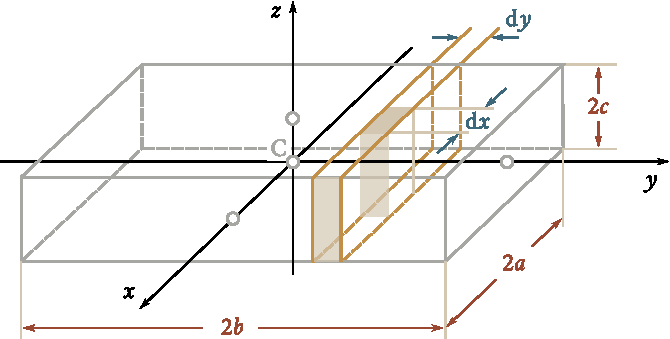
\includegraphics[scale=0.8]{figures/ch_05/fig_5_17.pdf}
		\caption[]{}
		\label{fig:5_17}
	\end{center}
\end{figure}

%Let us find the components of the inertia tensor for a homogeneous rectangular parallelepiped. We select the coordinate axes as shown in \fig{5_17}. The origin of coordinates coincides with the centre of mass of the body C. To calculate the axial moment of inertia $I_{zz}$ we divide our parallelepiped into columns with a base area of $\deriv{x}\,\deriv{y}$. All the elements of such a column have identical values of the coordinates $x$ and $y$. The volume of a column is $2c\,\deriv{x}\,\deriv{y}$, and its mass $\deriv{m}$ is $\rho 2c\,\deriv{x}\,\deriv{y}$. Therefore, the contribution of the column to $I_{zz}$ is determined by the expression
Ta hãy tìm các thành phần của tensor quán tính đối với một hình hộp chữ nhật bằng cách chọn các trục tọa độ như được vẽ trên \fig{5_17}. Gốc tọa độ trùng với khối tâm C của vật. Để tính moment quán tính trục $I_{zz}$, ta chia vật thành các cột nhỏ với diện tích đáy bằng $\deriv{x}\,\deriv{y}$. Tất cả các phần tử của cột này có các giá trị của các tọa độ $x$ và $y$ như nhau. Thể tích của cột bằng $2c\,\deriv{x}\,\deriv{y}$, còn khối lượng $\deriv{m}$ của nó bằng $\rho 2c\,\deriv{x}\,\deriv{y}$. Do đó, sự tham gia của cột vào $I_{zz}$ được định bằng biểu thức
\begin{equation*}
\deriv{I_{zz,\text{column}}} = 2\rho c(x^2+y^2)\deriv{x}\,\deriv{y}.
\end{equation*}

\noindent
%Integration of this expression with respect to $x$ gives the contribution to $I_{zz}$ of the layer of length $2a$, width $2c$, and thickness $\deriv{y}$ shown in \fig{5_17}:
Lấy tích phân biểu thức này theo $x$ ta tìm được sự tham gia vào $I_{zz}$ của một lớp có chiều dài $2a$, rộng $2c$ và dày $\deriv{y}$ như được biểu diễn ở \fig{5_17}:
\begin{align}
\deriv{I_{zz,\text{layer}}} &= \int_{-a}^{+a} 2\rho c(x^2+y^2)\,\deriv{x}\,\deriv{y}\nonumber\\
&= 2\rho c\,\deriv{y}\int_{-a}^{+a} x^2\,\deriv{x} + 2\rho cy^2\,\deriv{y}\int_{-a}^{+a}\deriv{x} \nonumber\\
&= \left(\frac{4}{3}\rho ca^3 + 4\rho cay^2\right)\,\deriv{y}\label{eq:5_42}
\end{align}

\noindent
%(the density $\rho$ does not depend on the coordinates $x$, $y$, and $z$ because the body is homogeneous).
(vì vật đồng nhất nên $\rho$ không phụ thuộc vào các tọa độ $x$, $y$, và $z$)

%Finally, integrating \eqn{5_42} with respect to $y$, we get $I_{zz}$ for the entire parallelepiped of mass $m$:
Cuối cùng, sau khi lấy tích phân \eqn{5_42} theo $y$, ta thu được $I_{zz}$ của toàn hình hộp chữ nhật khối lượng $m$ bằng:
\begin{align*}
I_{zz} &= \int_{-b}^{+b} \left(\frac{4}{3}\rho ca^3+4\rho cay^2\right)\,\deriv{y} = \frac{4}{3}\rho ca^3 \int_{-b}^{+b}\deriv{y} + 4\rho ca \int_{-b}^{+b} y^2 \,\deriv{y}\\
&= \frac{8}{3}\rho ca^3b + \frac{8}{3}\rho cab^3 = \frac{1}{3} \rho (2a)(2b)(2c)(a^2+b^2) = \frac{1}{3}m(a^2+b^2).
\end{align*}

\noindent
%Similar calculations give $I_{xx}=m(b^2+c^2)/3$, and $I_{yy}=m(a^2+c^2)/3$.
Các phép tính tương tự cho $I_{xx}=m(b^2+c^2)/3$, và $I_{yy}=m(a^2+c^2)/3$

%Now let us calculate one of the centrifugal moments, for instance $I_{xy}$. The contribution to this moment of a column with the base $\deriv{x}\,\deriv{y}$ is
Giờ ta hãy tính một trong những moment ly tâm, chẳng hạn như $I_{xy}$. Sự tham gia vào moment này của một cột diện tích đáy $\deriv{x}\,\deriv{y}$ bằng:
\begin{equation*}
\deriv{I_{xy,\text{column}}} = -\rho xy2c\,\deriv{x}\,\deriv{y}
\end{equation*}

\noindent
%and the contribution of a layer is
còn sự tham gia của lớp là
\begin{equation*}
\deriv{I_{xy,\text{layer}}} = -2\rho cy\,\deriv{x} \int_{-a}^{+a}x\,\deriv{y} = 0.
\end{equation*}

\noindent
%Accordingly, the moment of the entire parallelepiped equals zero. A similar result is also obtained for the other centrifugal moments. Thus, when we choose the coordinate axes as shown in \fig{5_17}, the inertia tensor of a homogeneous rectangular parallelepiped has the form
Một cách tương tự, moment quán tính của toàn bộ hình hộp bằng không. Kết quả tương tự thu được đối với cả trục tọa độ đã chỉ trên \fig{5_17}, tensor quán tính của một vật dạng hình chữ nhật đồng nhất có dạng
\begin{equation}\label{eq:5_43}
	I = \begin{pmatrix}
		I_x&0&0\\
		0&I_y&0\\
		0&0&I_z
	\end{pmatrix}
\end{equation}

\noindent
%(we have retained only one of the two identical subscripts for the diagonal components).
(ta đã giữ lại ở các thành phần chéo một chỉ số)

\begin{figure}[!htb]
	\begin{center}
		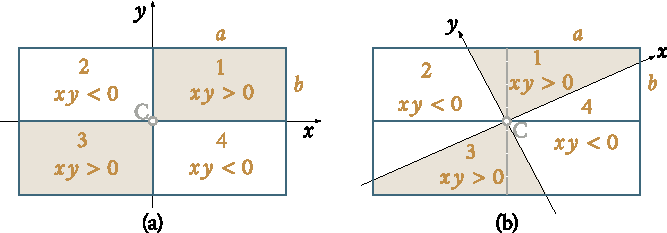
\includegraphics[scale=0.9]{figures/ch_05/fig_5_18.pdf}
		\caption[]{}
		\label{fig:5_18}
	\end{center}
\end{figure}

%We obtained such a result because we choose the principal axes of inertia (see Sec.~\ref{sec:5_3}) of the parallelepiped as the coordinate axes. Upon a different choice of the coordinate axes, the centrifugal moments of inertia will differ from zero. The following reasoning will convince us that this is true. When we choose the axes as shown in \fig{5_18}a, the areas of rectangles $1, 2, 3$, and $4$ are the same. On two of them, the product $xy$ is positive, and on two negative. As a result, the integral of $xy$ taken over the entire area vanishes. When we choose the axes as shown in \fig{5_18}b, the areas of the shaded figures $1$ and $3$ are less than those of the unshaded figures $2$ and $4$ (because $a>b$). Therefore, the integral of $xy$ taken over the entire area will differ from zero. Accordingly, the centrifugal moment $I_{xy}$ also differs from zero.
Ta thu được kết quả đó là do các trục quán tính chính của vật đã được chọn làm các trục tọa độ (xem phần ~\ref{sec:5_3}). Với cách chọn các trục tọa độ khác các moment quán tính ly tâm là khác không. Ở đây có thể thấy rõ nhờ lập luận sau. Khi chọn các trục được vẽ trên \fig{5_18}a, các diện tích của các hình chữ nhật $1, 2, 3,$ và $4$ là như nhau. Ở hai hình, trong chúng tích số $xy$ là dương, còn ở hai hình kia là âm. Điều này dẫn đến việc tích phân của $xy$ theo toàn bộ diện tích bằng không. Khi chọn các trục vẽ trên hình \fig{5_18}b, diện tích của các hình được tô đậm $1$ và $3$ nhỏ hơn diện tích của các hình không tô đậm $2$ và $4$ (vì $a>b$). Do đó tích phân của $xy$ lấy theo diện tích tổng cộng sẽ khác không. Một cách tương ứng, momen ly tâm $I_{xy}$ cũng khác không.

%The result obtained is common for all bodies regardless of their shape and mass distribution. If we take the principal axes of inertia of a body as the coordinate axes, the inertia tensor has the form given by \eqn{5_43}. The quantities $I_x, I_y, I_z$ [but not $I_{xx}, I_{yy}, I_{zz}$ in \eqn{5_34}; upon rotation of the coordinate axes all the tensor components change, the diagonal ones included] are called the \textbf{principal moments of inertia} of a body. It must be underlined that the axial moments calculated not about arbitrary axes, but about the principal ones, are called the principal moments of inertia.
Kết quả thu được là tổng quát đối với tất cả các vật, bất kể hình dạng và phân bố khối lượng của chúng như thế nào. Nếu ta lấy các trục quán tính chính của vật làm các trục tọa độ thì tensor quán tính có dạng \eqn{5_43}. Các đại lượng $I_x, I_y, I_z$ (nhưng không phải là $I_{xx}, I_{yy}, I_{zz}$ trong \eqn{5_34}; khi quay các trục tọa độ, tất cả các thành phần của tensor đều biến đổi, kể cả các thành phần chéo) được gọi là các \textbf{moment quán tính chính} của vật. Ta nhấn mạnh rằng những moment trục được tính theo các trục chính, mà không phải theo các trục tùy ý, thì được gọi là các moment quán tính chính.

%The principal axes of inertia are mutually perpendicular and intersect at the centre of mass of a body. In the general case (when $I_x\neq I_y\neq I_z$), we can choose these axes in a single way. For a spherical top (\ie, a body for which $I_x=I_y=I_z$, see Sec.~\ref{sec:5_3}), the position of the principal axes is absolutely indeterminate. For a symmetrical top ($I_x=I_y\neq I_z$), only the $z$-axis is fixed, the other two axes being indeterminate.
Các trục quán tính chính thì vuông góc với nhau và cắt nhau ở khối tâm của vật. Trong trường hợp tổng quát (khi $I_x\neq I_y\neq I_z$), ta có thể chọn các trục này theo một cách duy nhất. Đối với một con quay cầu (tức là một vật có$I_x=I_y=I_z$, xem phần ~\ref{sec:5_3}), vị trí của các trục chính là hoàn toàn không xác định. Ở con quay đối xứng ($I_x=I_y\neq I_z$), chỉ có trục $z$ được xác định, hai trục còn lại không xác định.

%Assume that a body rotates about one of its principal axes of inertia, say about the $z$-axis. Selecting the principal axes as the coordinate ones, we have $\omega_z=\omega, \omega_x=\omega_y=0$. Since the inertia tensor has the form of \eqn{5_43} when the coordinate axes are chosen in this way, Eqs.~\eqref{eq:5_30} give the following values of the components of the angular momentum of a body:
Giả sử một vật quay xung quanh một trong các trục quán tính chính của nó, chẳng hạn như quanh trục $z$. Khi chọn các trục chính làm các trục tọa độ, ta thu được $\omega_z=\omega, \omega_x=\omega_y=0$. Vì khi chọn các trục tọa độ như thế, tensor quán tính có dạng \eqn{5_43}, nên các công thức~\eqref{eq:5_30} dẫn tới các giá trị sau của các thành phần của moment động lượng của vật:
\begin{equation*}
L_x = L_y = 0,\quad L_z=I_z\omega.
\end{equation*}

\noindent
%Consequently, the vector $\vec{L}$ has the same direction as $\vec{\omega}$. The same result is obtained for rotation of a body about the other principal axes. In all these cases, we arrive at \eqn{5_12}:
Do đó, vector $\vec{L}$ có cùng hướng như $\omega$. Khi quay vật xung quanh các trục chính khác cũng thu được cùng kết quả đó. Trong tất cả các trường hợp đó
\begin{equation*}
\vec{L} = I\vec{\omega}
\end{equation*}

\noindent
%where $I$ is the corresponding principal moment of inertia of the body. In Sec.~\ref{sec:5_3}, we obtained \eqn{5_12} for a homogeneous body rotating about its axis of symmetry. Now we have established that this equation holds when an arbitrary body rotates about one of its principal axes of inertia.
trong đó $I$ là moment quán tính chính tương ứng của vật. Trong phần~\ref{sec:5_3}, ta đã thu được một công thức như thế cho một vật đồng nhất quay quanh trục đối xứng của nó (xem \eqn{5_12}). Bây giờ ta đã xác lập được rằng công thức trên là đúng trong các trường hợp mà một vật tùy ý quay xung quanh một trong các trục quán tính chính của nó.

%In conclusion, let us determine when the equation $\dot{\vec{L}}=\vec{M}$ [see \eqn{3_118}], which is always correct, can be written in the form
Để kết luận, ta hãy xác định xem trong những trường hợp nào thì công thức luôn đúng $\dot{\vec{L}}=\vec{M}$ (xem \eqn{3_118}) dưới dạng
\begin{equation}\label{eq:5_44}
I \vec{\alpha} = \vec{M}.
\end{equation}

%We may do this first of all when a body rotates about a principal axis, and the moment of the forces $\vec{M}$ is directed along this axis. Indeed, in this case, the moment $\vec{M}$ produces the increment $\deriv{\vec{L}}$ that is collinear with $\vec{L}$ ($\deriv{\vec{L}}=\vec{M}\,\deriv{t}$). Hence, rotation constantly takes place about a principal axis so that the relation $\vec{L}=I\vec{\omega}$ is never violated. In this case, however, \eqn{5_44} gives nothing new in comparison with the formula
Trước hết, rõ ràng có thể viết như vậy khi vật đang quay xung quanh trục chính, và moment $\vec{M}$ của các lực hướng dọc theo trục này. Thực vậy, trong trường hợp này moment $\vec{M}$ tạo ra số gia $\deriv{\vec{L}}$ đồng phương với $\vec{L}$ ($\deriv{\vec{L}}=\vec{M}\,\deriv{t}$). Vì vậy sự quay luôn luôn xảy ra xung quanh trục chính sao cho hệ thức $\vec{L}=I\vec{\omega}$ không bị vi phạm. Tuy nhiên trong trường hợp này công thức vector \eqn{5_44} không cho điều gì mới mẻ hơn so với công thức
\begin{equation}\label{eq:5_45}
	I\alpha_z = M_z.
\end{equation}

\noindent
%Here $z$ is the axis of rotation.
(ở đây $z$ là trục quay)

%When $\vec{M}$ is not collinear with $\vec{L}$ (for example, when $\vec{M}$ is perpendicular to $\vec{L}$, the axis of rotation moves relative to the body with time. Consequently, even provided that the relation $\vec{L}=I\vec{\omega}$ is obeyed at the initial moment, this relation stops being obeyed with time, and \eqn{5_44} loses its meaning. The displacement of the axis of rotation relative to the body is of no significance only when the body is a spherical top. For such a top, any axis is a principal one and has the same value of the moment of inertia $I$. Therefore, \eqn{5_44} holds for any mutual direction of the vectors $\vec{M}$ and $\vec{\omega}$.
Khi $\vec{M}$ không đồng phương với $\vec{L}$ (ví dụ như, khi $\vec{M}$ vuông góc với $\vec{L}$), thì trục quay dịch chuyển đối với vật theo thời gian. Do đó ngay cả khi hệ thức $\vec{L}=I\vec{\omega}$ đúng tại thời điểm ban đầu, theo thời gian nó sẽ không được tuân theo nữa, và \eqn{5_44} mất ý nghĩa của nó. Chỉ trong trường hợp khi vật là con quay cầu thì sự dịch chuyển trục quay đối với vật mới không quan trọng. Đối với con quay cầu, một trục bất kì là trục chính và moment quán tính $I$ có các giá trị như nhau. Do đó, phương trình \eqn{5_44} giữ vững đối với một hướng tương hỗ bất kì của các vector $\vec{M}$ và $\vec{\omega}$.

\begin{figure}[!htb]
	\begin{center}
		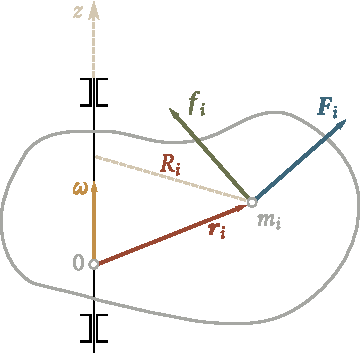
\includegraphics[scale=1]{figures/ch_05/fig_5_19.pdf}
		\caption[]{}
		\label{fig:5_19}
	\end{center}
\end{figure}

\section{Động năng của vật rắn quay}\label{sec:5_6}

%Let us begin with a consideration of the rotation of a body about a fixed axis, which we shall call the $z$-axis (\fig{5_19}). The linear velocity of the elementary mass $m_i$ is $v_i=\omega R_i$ where $R_i$ is the distance from the mass $m_i$ to the $z$-axis. Consequently, we get the following expression for the kinetic energy of the $i$-th elementary mass:
Ta bắt đầu nghiên cứu sự quay một vật xung quanh một trục cố định mà ta gọi là trục $z$ (\fig{5_19}). Vận tốc dài của khối lượng nguyên tố $m_i$ bằng $v_i=\omega R_i$ trong đó $R_i$ là khoảng cách từ trục $z$ đến khối lượng $m_i$. Do đó, ta thu được biểu thức cho động năng của khối lượng nguyên tố thứ $i$
\begin{equation*}
	E_{\text{k},i} = \frac{m_i v_i^2}{2} = \frac{1}{2}m_i \omega^2 R_i^2.
\end{equation*}

\noindent
%The kinetic energy of a body is composed of the kinetic energies of its parts:
Động năng của vật được tạo thành từ động năng của các phần của nó:
\begin{equation*}
	E_{\text{k}} = \sum_i E_{\text{k},i} = \frac{1}{2}\omega^2 \sum_i m_i R_i^2.
\end{equation*}

\noindent
%The sum in the right-hand side of this equation is the moment of inertia of the body $I_z$ relative to the axis of rotation. The kinetic energy of a body rotating about a fixed axis thus equals
Tổng ở vế phải của hệ thức này là moment quán tính $I_z$ của vật đối với trục quay. Như vậy động năng của vật quay quanh một trục cố định bằng
\begin{equation}\label{eq:5_46}
	E_{\text{k}} = \frac{1}{2} I_z \omega^2.
\end{equation}

%Assume that the mass $m_i$ experiences\footnote{The resultant force $\vec{f}_i+\vec{F}_i$ is in a plane perpendicular to the axis of rotation.} the internal force $\vec{f}_i$, and the external force $\vec{F}_i$ (see \fig{5_19}). According to \eqn{3_16}, these forces do the following work during the time $\deriv{t}$:
Giả sử nội lực $$\vec{f}_i$$ và ngoại lực $$\vec{F}_i$$ (xem \fig{5_19}) tác dụng\footnote{Lực tổng hợp $\vec{f}_i+\vec{F}_i$ nằm trong mặt phẳng vuông góc với trục quay.} lên khối lượng $m_i$. Theo \eqn{3_16}, các lực này trong thời gian $\deriv{t}$ thực hiện công sau:
\begin{equation*}
\deriv{A_i} = \vecdotind{f}{i}{v}{i}\,\deriv{t} + \vecdotind{F}{i}{v}{i}\,\deriv{t} = \vec{f}_i\boldsymbol{\cdot}(\vecprod{\omega}{r}_i)\,\deriv{t} + \vec{F}_i\boldsymbol{\cdot}(\vecprod{\omega}{r}_i)\,\deriv{t}.
\end{equation*}

\noindent
%Performing a cyclic transposition of the multipliers in the scalar triple products [see \eqn{1_34}] we get
Thực hiện phép hoán vị vòng quanh lên các thừa số trong các tích hỗn hợp vector (xem \eqn{1_34}), ta được
\begin{equation}\label{eq:5_47}
\deriv{A_i} = \vec{\omega}\,\boldsymbol{\cdot}(\vecprodind{r}{i}{f}{i})\,\deriv{t} + \vec{\omega}\boldsymbol{\cdot}(\vecprodind{r}{i}{F}{i})\,\deriv{t} = \vecdot{\omega}{M}_{\text{int},i}\,\deriv{t} + \vecdot{\omega}{M}_i\,\deriv{t}
\end{equation}

\noindent
%where $\vec{M}_{\text{int},i}$ is the moment of an internal force relative to point $0$, and $\vec{M}_i$ is the similar moment of an external force.
trong đó $\vec{M}_{\text{nội},i}$ là moment của nội lực đối với điểm $0$, và $\vec{M}_i$ là moment tương tự của ngoại lực.

%Summation of \eqn{5_47} for all the elementary masses yields the elementary work done on the body during the time $\deriv{t}$:
Lấy tổng biểu thức \eqn{5_47} theo tất cả khối lượng nguyên tố ta thu được công nguyên tố thực hiện trên vật trong thời gian $\deriv{t}$:
\begin{equation*}
	\deriv{A} = \sum_i \deriv{A}_i = \vec{\omega}\left(\sum_i \vec{M}_{\text{nội},i}\right)\,\deriv{t} + \vec{\omega}\left(\sum_i \vec{M}_{i}\right)\,\deriv{t}.
\end{equation*}

\noindent
%The sum of the moments of the internal forces equals zero [see \eqn{3_117}]. Consequently, designating the total moment of the external forces by $\vec{M}$, we get the expression
Tổng các moment của các nội lực là bằng không (xem \eqn{3_117}). Do đó, nếu ký hiệu tổng các moment ngoại lực bằng $\vec{M}$, ta viết được biểu thức:

\begin{equation}\label{eq:5_48}
	\deriv{A} = \vecdot{\omega}{M}\,\deriv{t} = \omega M_z\,\deriv{t}
\end{equation}

\noindent
%[we have used \eqn{1_21}, taking into account that $M_{\omega} = M_z$]. Finally, since $\omega\,\deriv{t}$ is the angle $\deriv{\varphi}$ through which the body turns during the time $\deriv{t}$, we have
(ta đã sử dụng \eqn{1_21}, thấy rằng $M_{\omega} = M_z$). Cuối cùng, để ý rằng $\omega\,\deriv{t}$ chính là góc $\deriv{\varphi}$ mà vật quay được trong $\deriv{t}$, ta có:
\begin{equation}\label{eq:5_49}
	\deriv{A} = M_z\,\deriv{\varphi}.
\end{equation}

\noindent
%The sign of the work depends on that of $M_z$, \ie, on the sign of the projection of the vector $\vec{M}$ onto the direction of the vector $\vec{\omega}$.
Dấu của công phụ thuộc vào dấu của $M_z$, tức là dấu của hình chiếu của $\vec{M}$ lên hướng của $\vec{\omega}$.

%Thus, internal forces do no work when a body rotates, the work of the external forces is determined by \eqn{5_49}. We can arrive at \eqn{5_49} by taking advantage of the fact that the work done by all the forces applied to a body goes to increase its kinetic energy [see \eqn{3_11}]. Differentiating both sides of \eqn{5_46}, we obtain
Vậy khi quay vật, các nội lực không thực hiện công, còn công của các ngoại lực được xác định bằng \eqn{5_49}. Ta có thể đi tới \eqn{5_49} nếu khai thác tính chất là công thực hiện bởi tất cả các lực đặt lên vật làm tăng động năng của nó (xem \eqn{3_11}). Vi phân cả hai vế của \eqn{5_46}, ta thu được
\begin{equation*}
	\deriv{E_{\text{k}}} = I_z\omega\,\deriv{\omega} = I_z\omega\dot{\omega}\,\deriv{t}.
\end{equation*}

\noindent
%According to \eqn{5_15}, $I_z\dot{\omega}=M_z$, and the product $\omega\,\deriv{t}$ equals $\deriv{\varphi}$. Hence, substituting $\deriv{A}$ for $\deriv{E_{\text{k}}}$ we arrive at \eqn{5_49}.
Theo \eqn{5_15}, $I_z\dot{\omega}=M_z$, và tích $\omega\,\deriv{t}$ bằng $\deriv{\varphi}$. Do đó, thế $\deriv{A}$ vào $\deriv{E_{\text{k}}}$ ta được \eqn{5_49}.

%Table~\ref{table:5_1} compares the formulas of mechanics of rotation with similar formulas of mechanics of translation (mechanics of a particle). This comparison shows that in all cases of rotation the part of mass is played by the moment of inertia, the part of force by the moment of a force, the part of momentum by the angular momentum, and so on.
Trong bảng~\ref{table:5_1} người ta so sánh các công thức của chuyển động quay với các công thức tương đương của chuyển động tịnh tiến (cơ học chát điểm). Từ sự so sánh này dễ dàng kết luận rằng trong mọi trường hợp, moment quán tính đóng vai trò của khối lượng, moment lực đóng vai trò của lực, moment động lượng đóng vai trò của động lượng, v.v...

\begin{table}[!htb]
	\renewcommand{\arraystretch}{1.2}
	\caption{}
	\label{table:5_1}
	\begin{center}\resizebox{0.92\linewidth}{!}{
			\begin{tabular}{ll}
				\toprule[1pt]
				%\textbf{Translation} & \textbf{Rotation}\\
                \textbf{Tịnh tiến} & \textbf{Quay}\\
				\midrule[0.5pt]\midrule[0.5pt]
				$\vec{v} =\,$ vận tốc tịnh tiến & $\vec{\omega} = \,$ vận tốc góc\\
				$\vec{a}=\dot{\vec{v}} =\,$ gia tốc tịnh tiến & $\vec{\alpha}=\dot{\vec{\omega}} =\,$ gia tốc góc\\
				$m=\,$ khối lượng & $I_z=\,$ moment quán tính\\
				$\vec{p}=m\vec{v}=\,$ động lượng & $L_z=I_z\omega=\,$ moment động lượng\\
				$\vec{F}=\,$ lực & $\vec{M}$ or $M_z=\,$ moment lực\\
				$\dot{\vec{p}}=\vec{F}$ & $\dot{\vec{L}}=\vec{M}$\\
				$m\vec{a}=\vec{F}$ & $I\alpha_z=M_z$\\
				$E_{\text{k}}=\frac{1}{2}mv^2$ & $E_{\text{k}}=\frac{1}{2}I\omega^2\,$ (đối với một trục quay cố định)\\
				$\deriv{A}=F_{s}\,\deriv{s}$ & $\deriv{A}=M_z\,\deriv{\varphi}$\\
				\bottomrule[1pt]
			\end{tabular}
	}\end{center}
\end{table}

%We obtained \eqn{5_46} for the case when a body rotates about a stationary axis fixed in the body. Now let us assume that a body rotates arbitrarily relative to a fixed point coinciding with its centre of mass. We shall rigidly associate a Cartesian system of coordinates with the body and place its origin at the centre of mass. The velocity of the $i$-th elementary mass is $\vec{v}_i=\vecprod{\omega}{r}_i$. Consequently, we can write the following expression for the kinetic energy of the body:
Ta đã thu được \eqn{5_46} cho trường hợp khi vật quay xung quanh trục cố định bên trong vật. Bây giờ ta giả sử rằng vật quay một cách tùy ý đối với một điểm cố định trùng với khối tâm của nó. Ta hãy gắn chặt với vật hệ tọa độ Descartes có gốc đặt tại khối tâm của vật. Vận tốc của khối lượng nguyên tố thứ $i$ bằng $\vec{v}_i=\vecprod{\omega}{r}_i$. Do đó, đối với động năng của vật có thể viết biểu thức:
\begin{equation*}
	E_{\text{k}} = \frac{1}{2}\sum_i m_iv_i^2 = \frac{1}{2}\sum_i m_i (\vecprod{\omega}{r}_i)^2 = \frac{1}{2}\sum_i m_i \omega^2 r_i^2\sin^2\varphi_i
\end{equation*}

\noindent
%where $\varphi_i$ is the angle between the vectors $\vec{\omega}$ and $\vec{r}_i$. Substituting $1-\cos^2\varphi_i$ for $\sin^2\varphi_i$, and taking into account that $\omega r_i\cos\varphi=\vecdot{\omega}{r}_i$, we have
trong đó $\varphi_i$ là góc giữa các vector $\vec{\omega}$ và $\vec{r}_i$. Thay $1-\cos^2\varphi_i$ bằng $\sin^2\varphi_i$, và để ý rằng $\omega r_i\cos\varphi=\vecdot{\omega}{r}_i$, ta có:
\begin{equation*}
	E_{\text{k}} = \frac{1}{2}\sum_i m_i [\vec{\omega}^2\vec{\cdot}\vec{r}_i^2 - (\vecdot{\omega}{r}_i)^2]^2.
\end{equation*}

\noindent
%Let us write out the scalar products through the projections of the vectors $\vec{\omega}$ and $\vec{r}_i$ onto the axes of the coordinate system associated with the body:
Ta viết tích vô hướng qua các hình chiếu của các vector $\vec{\omega}$ và $\vec{r}_i$ lên trục của hệ tọa độ gắn với vật:
\begin{align*}
	E_{\text{k}} &= \frac{1}{2}\sum_i m_i \left[(\omega_x^2+\omega_y^2+\omega_z^2)(x_i^2+y_i^2+z_i^2) \right.\\
	&\quad\quad\left. - (\omega_x x_i+\omega_y y_i+\omega_z z_i)(\omega_x x_i+\omega_y y_i+\omega_z z_i)\right]\\
	&= \frac{1}{2}\sum_i m_i \left[(\omega_x^2+\omega_y^2+\omega_z^2)(x_i^2+y_i^2+z_i^2)  \right.\\
	&\quad\quad\left. -\omega_x^2x_i^2 - \omega_x\omega_yx_iy_i - \omega_x\omega_zx_iz_i - \omega_y\omega_xy_ix_i - \omega_y^2y_i^2   \right.\\
	&\quad\quad\quad\left. - \omega_y\omega_zy_iz_i - \omega_z\omega_xz_ix_i - \omega_z\omega_yz_iy_i - \omega_z^2z_i^2\right].
\end{align*}

\noindent
%inally, combining addends with identical products of the angular velocity components and putting these products outside the sums, we get
Cuối cùng hợp nhất các số hạng có tích giống nhau của các thành phần vận tốc góc và đưa các tích này ra ngoài dấu tổng, ta được:

\begin{align*}
	E_{\text{k}} &= \frac{1}{2}\left[(\omega_x^2 \sum_i m_i (y_i^2+z_i^2) + \omega_y^2 \sum_i m_i (x_i^2+z_i^2) + \omega_z^2 \sum_i m_i (x_i^2+y_i^2) \right.\\
	&\quad\quad\left. - \omega_x\omega_y \sum_i m_ix_iy_i - \omega_x\omega_z \sum_i m_i x_iz_i - \omega_y\omega_x \sum_i m_i y_ix_i \right.\\
	&\quad\quad\quad\left. -\omega_y\omega_z \sum_i m_i y_iz_i - \omega_z\omega_x \sum_i m_i z_ix_i - \omega_z\omega_y \sum_i m_i z_iy_i\right].
\end{align*}

%The sums by which the products of the angular velocity components are multiplied are the components of the inertia tensor [see \eqn{5_41}]. Hence, we have arrived at the equation
Các tổng mà người ta nhân chúng với các tích của các thành phần của tensor quán tính (xem \eqn{5_41}). Do đó, ta đi tới công thức
\begin{align}
	E_{\text{k}} &= \frac{1}{2}\left[I_{xx}\omega_x^2 + I_{xy}\omega_x\omega_y + I_{xz}\omega_x\omega_z + I_{yx}\omega_y\omega_x \right.\nonumber\\
	&\quad\quad\left. + I_{yy}\omega_y^2 + I_{yz}\omega_y\omega_z + I_{zx}\omega_z\omega_x + I_{zy}\omega_z\omega_y + I_{zz}\omega_z^2\right].\label{eq:5_50}
\end{align}

\noindent
%This equation can be written in the form
Có thể viết công thức này dưới dạng
\begin{equation}\label{eq:5_51}
	E_{\text{k}} = \frac{1}{2}\sum_{i,k=x,y,z} I_{ik}\omega_i\omega_k.
\end{equation}

\noindent
%In summation, the subscripts $i$ and $k$ are sequentially given the values $x, y, z$ independently of each other.
Khi lấy tổng, các chỉ số $i$ và $k$ lấy các giá trị $x, y, z$ một cách độc lập với nhau

%If the axes of a coordinate system associated with a body are chosen so that they coincide with the principal axes of inertia of the body, the centrifugal moments of inertia will vanish, and \eqn{5_50} will become simplified as follows:
Nếu chọn các trục của hệ tọa độ gắn với vật sao cho chúng trùng với các trục quán tính chính của vật thì các moment quán tính ly tâm triệt tiêu và \eqn{5_50} được đơn giản hóa như sau:
\begin{equation}\label{eq:5_52}
	E_{\text{k}} = \frac{1}{2}(I_x\omega_x^2 + I_y\omega_y^2 + I_z\omega_z^2).
\end{equation}

\noindent
%Here $I_x, I_y, I_z$ are the principal moments of inertia of the body. For a spherical top, these moments have the identical value I so that \eqn{5_52} becomes $E_{\text{k}}=I\omega^2/2$ [compare with \eqn{5_46}]. When an arbitrary body rotates about one of the principal axes of inertia, say the $z$-axis, we have $\omega_z=\omega, \omega_x\omega_y=0$, and \eqn{5_52} transforms into~\eqn{5_46}. Thus, the kinetic energy of a rotating body equals half the product of the moment of inertia and the square of the angular velocity in three cases: (1) for a body rotating about a fixed axis, (2) for a body rotating about one of the principal axes of inertia, and (3) for a spherical top. In all other cases, the kinetic energy is determined by more complicated equations~\eqref{eq:5_50} or \eqref{eq:5_52}.
Ở đây $I_x, I_y, I_z$ là các moment quán tính chính của vật. Đối với một con quay cầu, các moment này có cùng độ lớn $I$, cho nên \eqn{5_52} có dạng $E_{\text{k}}=I\omega^2/2$ (so sánh với \eqn{5_46}). Khi quay một vật tùy ý xung quanh một trong các trục quán tính chính, chẳng hạn trục $z$, ta có $\omega_z=\omega, \omega_x\omega_y=0$, và \eqn{5_52} chuyển thành~\eqn{5_46}.
Như vậy, động năng của một vật quay là bằng nửa tích của moment quán tính với bình phương vận tốc góc trong ba trường hợp: 1) đối với một vật quay xung quanh một trục cố định, 2) đối với một vật quay xung quanh một trong các trục quán tính chính, 3) đối với một con quay cầu. Trong các trường hợp còn lại động năng được xác định bằng các công thức phức tạp hơn là~\eqref{eq:5_50} hoặc \eqref{eq:5_52}.

\section{Động năng của vật trong chuyển động phẳng}\label{sec:5_7}

\vspace{-5pt}

%The plane motion of a body can be represented as the superposition of two mo\-tions---translation with a velocity $\vec{v}_0$ and rotation about the relevant axis with the angular velocity $\vec{\omega}$ (see Sec.~\ref{sec:5_1}). By \eqn{5_1}, the velocity of the $i$-th elementary mass of a body is
Chuyển động phẳng của một vật có thể được biểu diễn như sự cộng hai chuyển động là chuyển động tịnh tiến với một vận tốc $\vec{v}_o$ nào đó và sự quay xung quanh một trục tương ứng với vận tốc góc $\vec{\omega}$ (xem phần~\ref{sec:5_1}). Theo \eqn{5_1}, vận tốc của khối lượng nguyên tố thứ $i$ của vật sẽ bằng
\begin{equation*}
	\vec{v}_i = \vec{v}_0 + \vecprod{\omega}{r}_i
\end{equation*}

\noindent
%where $\vec{v}_0$ is the velocity of a certain point $0$ of the body, and $\vec{r}_i$ is the position vector determining the position of the elementary mass with respect to point $0$.
trong đó $\vec{v}_o$ là vận tốc của một điểm $O$ nào đó của vật, $\vec{r}_i$ là vector bán kính xác định vị trí của khối lượng nguyên tố đó đối với $O$.

%The kinetic energy of the $i$-th elementary mass is
Động năng của khối lượng nguyên tố thứ $i$ sẽ bằng
\begin{equation*}
	E_{\text{k},i} = \frac{1}{2}m_i v_i^2 = \frac{1}{2}m_i (\vec{v}_0 + \vecprod{\omega}{r}_i)^2.
\end{equation*}

\noindent
%Squaring the expression in parenthesis, we get
Bình phương biểu thức, ta được:
\begin{equation*}
	E_{\text{k},i} = \frac{1}{2}m_i \left[v_0^2 + 2\vec{v}_0\vec{\cdot}(\vecprod{\omega}{r}_i) + (\vecprod{\omega}{r}_i)^2\right].
\end{equation*}

\noindent
%The vector product of $\vec{\omega}$ and $\vec{r}_i$ has a magnitude equal to $\omega R_i$, where $R_i$ is the distance to the mass $m_i$ from the axis of rotation [see \fig{1_33} and the text preceding \eqn{1_100}]. Consequently, the third addend in the brackets equals $\omega^2R_i^2$. Let us perform a cyclic transposition of the multipliers in the second addend [see \eqn{1_34}]. As a result, we obtain
Tích vector của $\vec{\omega}$ và $\vec{r}_i$ có module bằng $\omega R_i$, trong đó $R_i$ là khoảng cách tính từ khối lượng $m_i$ tới trục quay (xem \fig{1_33} và đoạn ngay trước \eqn{1_100}). Do đó, số hạng thứ ba trong các dấu ngoặc bằng $\omega^2R_i^2$. Ta hãy thực hiện phép hoán vị vòng quanh cho các thừa trong số hạng thứ hai (xem \eqn{1_34}). Kết quả thu được biểu thức:
\begin{equation}\label{eq:5_53}
	E_{\text{k},i} = \frac{1}{2}m_i \left[v_0^2 + 2(\vec{v}_0\times\vec{\omega})\vec{\cdot}\vec{r}_i + \omega^2 R_i^2\right].
\end{equation}

%To obtain the kinetic energy of a body, we find the sum of \eqn{5_53} for all the elementary masses, putting the constant factors outside the sum:
Để thu được động năng của vật, ta lấy tổng biểu thức \eqn{5_53} cho tất cả các khối lượng nguyên tố, hơn nữa đặt các thừa số không đổi ra ngoài phép tổng:
\begin{equation*}
	E_{\text{k}} = \frac{1}{2} v_0^2 \sum_i m_i + (\vec{v}_0\times\vec{\omega})\vec{\cdot}\sum_i m_i\vec{r}_i + \frac{1}{2}\omega^2 \sum_i m_iR_i^2.
\end{equation*}

\noindent
%The sum of the elementary masses $\sum_i m_i$ is the mass of the body $m$. The expression $\sum_i m_i\vec{r}_i$ is the product of the mass of the body and the position vector $\vec{r}_{\text{C}}$ of the centre of mass of the body. Finally, $\sum_i m_iR_i^2$ is the moment of inertia of the body $I_0$ relative to an axis passing through point $0$. We can therefore write that
Tổng các khối lượng nguyên tố $\sum_i m_i$ là khối lượng $m$ của vật. Biểu thức $\sum_i m_i\vec{r}_i$ bằng tích khối lượng của vật với bán kính vector $\vec{r}_{\text{C}}$ của khối tâm của vật. Cuối cùng, $\sum_i m_iR_i^2$ là moment quán tính $I_O$ của vật đối với một trục đi qua điểm $O$. Do đó, có thể viết
\begin{equation}\label{eq:5_54}
	E_{\text{k}} = \frac{1}{2} mv_0^2 + m\vec{r}_{\text{C}}\vec{\cdot}(\vec{v}_0\times\vec{\omega}) + \frac{1}{2} I_0\omega^2.
\end{equation}

%If we take the centre of mass of the body as point $0$, the position vector $\vec{r}_{\text{C}}$ will equal zero, and the second addend will vanish. Consequently, designating by $\vec{v}_{\text{C}}$ the velocity of the centre of mass, and by $I_{\text{C}}$ the moment of inertia of the body relative to an axis passing through point C, we get the following expression for the kinetic energy of the body:
Nếu lấy khối tâm $C$ của vật làm điẻm $O$ thì bán kính $\vec{r}_{\text{C}}$ sẽ bằng không, cho nên số hạng thứ hai sẽ biến mất. Do đó, khi ký hiệu vận tốc của khối tâm là $\vec{v}_{\text{C}}$, còn moment quán tính của vật đối với trục quay đi qua điểm $C$ là $I_C$, ta thu được công thức đối với động năng của vật:
\begin{equation}\label{eq:5_55}
	E_{\text{k}} = \frac{1}{2}m v_{\text{C}}^2 + \frac{1}{2} I_{\text{C}} \omega^2.
\end{equation}

%Thus, the kinetic energy of the body in plane motion consists of the energy of translation with a velocity equalling that of the centre of mass and the energy of rotation about an axis passing through the centre of mass of the body.
Như vậy, động năng của vật trong chuyển động phẳng được tạo thành từ năng lượng chuyển động tịnh tiến với vận tốc bằng vận tốc khối tâm và năng lượng quay xung quanh trục đi qua khối tâm của vật.

\section{Ứng dụng các định luật động lực học vật rắn}\label{sec:5_8}

%The motion of a rigid body is described by two equations (\eqref{eq:5_6} and \eqref{eq:3_118}) that have already been given in previous sections:
Chuyển động của vật rắn được mô tả bằng hai phương trình đã được chứng minh từ trước (xem \eqref{eq:5_6} và \eqref{eq:3_118}):
\begin{align*}
	m\vec{a}_{\text{C}} &= \sum\vec{F}_{\text{ng}}\\
	\dot{\vec{L}} &= \sum\vec{M}_{\text{ng}}.
\end{align*}

\noindent
%The motion of a body is thus determined by the external forces and the moments of these forces acting on it.
Do đó, chuyển động của vật được xác định bởi các ngoại lực tác dụng lên vật và các moment của các lực này.


\begin{figure}[!htb]
	\begin{center}
		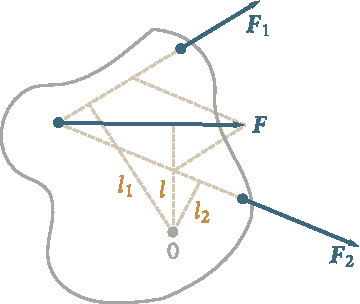
\includegraphics[scale=0.95]{figures/ch_05/fig_5_20.pdf}
		\caption[]{}
		\label{fig:5_20}
	\end{center}
\end{figure}

%The moments of the forces may be taken relative to any point that is stationary or moving without acceleration. If we took the moment of the external forces relative to a point moving with acceleration, we would in essence write \eqn{3_118} in a non-inertial reference frame. In this case, we must take into consideration the forces of inertia and their moments apart from the external forces due to the interaction of the given body with other bodies.
Có thể lấy các moment của các lực đối với một điểm bất kỳ đứng yên hoặc chuyển động không có gia tốc. Khi lấy moment của các ngoại lực đối với một điểm chuyển động có gia tốc thì, về bản chất, ta đã viết \eqn{3_118} trong hệ quy chiếu không quán tính. Trong trường hợp này, ngoài các ngoại lực được gây bởi tương tác của vật đã cho với các vật khác, cần phải tính đến các lực quán tính và các moment của chúng.

%The points of application of the forces acting on a body may be transferred along the lines of action of the forces because neither the sum of the forces nor their moments will change when this is done (when a force is transferred along the line of its action, the moment arm relative to any point remains unchanged). This permits us to replace several forces with a single one equivalent to them in its action on a body. For example, the two forces $\vec{F}_1$ and $\vec{F}_2$ in one plane (\fig{5_20}) may be replaced with the force $\vec{F}$ equivalent to them. The point of application of the latter may also be chosen arbitrarily on the direction of its action.
Có thể dịch chuyển các điểm đặt của các lực tác dụng lên vật dọc theo các đường tác dụng của các lực, vì khi đó không có tổng các lực nào hoặc các moment nào của các lực bị biến đổi (khi dịch chuyển lực dọc theo đường tác dụng của nó, cánh tay đòn đối với một điểm bất kì vẫn không biến đổi). Điều này cho phép thay thế một số lực bằng một lực tương đương với chúng đối với tác động gây ra cho vật. Chẳng hạn, có thể thay thế hai lực $\vec{F}_1$ và $\vec{F}_2$ nằm trong một mặt phẳng (\fig{5_20}) bằng một lực $\vec{F}$ tương đương, mà cũng có thể tuỳ ý chọn điểm đặt của nó trên phương dọc theo đó nó tác dụng.

%A combination of parallel forces acting on a body may be replaced with their resultant equal to the sum of all the forces and applied to a point of the body such that its moment equals the sum of the moments of the separate forces.
Có thể thay thế tập hợp các lực song song tác dụng lên vật bằng hợp lực của chúng; hợp lực này bằng tổng của tất cả các lực và đặt vào một điểm của vật sao cho moment của nó bằng tổng các moment của các lực riêng rẽ.

%Let us find the resultant of the forces of gravity. These forces are applied to all the elements of a body, the force $m_i\vec{g}$ acting on the elementary mass $m_i$. The sum of these forces is $\vec{P}=m\vec{g}$, where $m=\sum_im_i$ is the mass of the body. The total moment of the forces of gravity relative to a certain point $0$ is
Ta hãy thử tìm hợp lực của các trọng lực. Các lực này đặt vào mọi phần tử của vật, thêm vào đó lực $m_i\vec{g}$ tác dụng lên khối lượng nguyên tố $m_i$. Tổng các lực bằng $\vec{P}=m\vec{g}$, trong đó $m=\sum_im_i$ là khối lượng của vật. Moment tổng của các trọng lực đối với một điểm $O$ nào đó bằng
\begin{equation*}
	\vec{M} = \sum_i \vec{r}_i \times (m_i \vec{g})
\end{equation*}

\noindent
%where $\vec{r}_i$ is the position vector determining the position of the mass $m_i$ with respect to point $0$. Transferring the scalar multiplier $m_i$ from the second member of the product to the first one and then putting the common factor $\vec{g}$ outside the sum, we get
trong đó $\vec{r}_i$ là bán kính vector xác định vị trí của khối lượng $m_i$ đối với điểm $O$. Nếu chuyển thừa số vô hướng $m_i$ từ nhân tử thứ hai sang nhân tử thức nhất và sau đó đưa thừa số chung $g$ ra ngoài dấu tổng, ta được:
\begin{equation*}
	\vec{M} = \left(\sum_i m_i \vec{r}_i\right) \times \vec{g}.
\end{equation*}

\noindent
%The sum in parentheses equals the product of the mass of the body and the position vector $\vec{r}_{\text{C}}$ of the centre of mass C. Hence,
Tổng đứng trong các dấu ngoặc tròn bằng tích khối lượng của vật với bán kính vector $\vec{r}_{\text{C}}$ của khối tâm $C$. Do đó
\begin{equation}\label{eq:5_56}
	\vec{M} = (m\vec{r})\times\vec{g} = \vec{r}_{\text{C}} \times (m\vec{g}) = \vec{r}_{\text{C}} \times \vec{P}.
\end{equation}

\noindent
%Thus, the total moment of the forces of gravity relative to an arbitrary point $0$ coincides with the moment of the force $m\vec{g}$ applied to point C. Thus, the resultant of the forces of gravity equals $\vec{P}=m\vec{g}$ and is applied to the centre of mass of the body. We must note that this holds only when the field of the forces of gravity is homogeneous within the body [in deriving \eqn{5_56} we considered that $\vec{g}=\text{constant}$].
Như vậy, moment tổng của các trọng lực đối với một điểm $O$ tuỳ ý trùng với moment của lực $m\vec{g}$ đặt vào điểm $C$. Như vậy hợp lực của các trọng lực bằng $\vec{P}=m\vec{g}$ và đặt vào khối tâm của vật. Ta lưu ý rằng điều này chỉ đúng trong trường hợp nếu trong phạm vi vật trọng trường là đều (khi rút ra công thức \eqn{5_56} ta đã coi rằng $\vec{g}=\text{constant}$)

%It follows from \eqn{5_56} that the moment of the forces of gravity relative to the centre of mass equals zero (in this case $\vec{r}_{\text{C}}=0$). The point relative to which the moment of the forces of gravity equals zero is called the \textbf{centre of gravity} of the body. Thus, when the field of gravity forces is homogeneous within a body, the centre of gravity coincides with the centre of mass.
Từ \eqn{5_56} suy ra rằng moment của các trọng lực đối với khối tâm là bằng không (trong trường hợp này $\vec{r}_{\text{C}}=0$). Điểm mà moment của các trọng lực đối với nó bằng không được gọi là \textbf{trọng tâm} của vật. Như vậy, trong trường hợp khi trọng trường trong phạm vi vật là đều, thì trọng tâm trùng với khối tâm.

%For a homogeneous gravitational field, the forces of gravity applied to different elementary masses have an identical direction and are proportional to $m_i$. The forces of inertia produced in a non-inertial reference frame moving in a straight line relative to inertial frames have the same property. Indeed, in this case, the forces of inertia applied to the elementary masses $m_i$ equal $-m_i\vec{a}_0$, where $\vec{a}_0$ is the acceleration of the non-inertial frame [see \eqn{4_2}]. By repeating the reasoning that led us to \eqn{5_56} (here $-m_i\vec{a}_0$ must be substituted for $m\vec{g}$), we can show that the resultant of the inertia forces equals $-m\vec{a}_0$ and is applied to the centre of mass of the body. It must be stressed that this holds only for reference frames moving in a straight line.
Trong trường hợp trọng trường đều các trọng lực đặt vào các khối lượng nguyên tố khác nhau đều có hướng như nhau và tỉ lệ với $m_i$. Các lực quán tính xuất hiện trong hệ quy chiếu không quán tính chuyển động tịnh tiến đối với các hệ quy chiếu quán tính cũng có tính chất như thế. Thật vậy, trong trường hợp này các lực quán tính đặt vào các khối lượng nguyên tố $m_i$ bằng $-m_i\vec{a}_0$, trong đó $\vec{a}_0$ là gia tốc của hệ không quán tính (xem \eqn{4_2}). Nếu lặp lại các lập luận đã dẫn đến công thức \eqn{5_56} (trong đó $-m_i\vec{a}_0$ cần thay thế cho $m\vec{g}$) thì có thể chứng tỏ rằng hợp lực của các lực quán tính bằng $-m_i\vec{a}_0$ và được đặt vào khối tâm của vật. Ta nhấn mạnh rằng, điều này chỉ đúng đối với các hệ quy chiếu chuyển động tịnh tiến.

%The moment of the inertia forces relative to the centre of mass equals zero (in a frame with translational motion). Therefore, when compiling \eqn{3_118} for the moments taken relative to the centre of mass, the forces of inertia do not have to be taken into consideration.
Moment của các lực quán tính (trong hệ quy chiếu chuyển động tịnh tiến) đối với khối tâm là bằng không. Do đó, khi thành lập phương trình \eqn{3_118} đối với các moment được lấy đối với khối tâm thì không cần tính tới lực quán tính.

%Let us find the conditions of equilibrium of a rigid body. A body can remain in a state of rest if nothing causes the appearance of translation or rotation. According to Eqs.~\eqref{eq:5_6} and \eqref{eq:3_118}, two conditions are essential and sufficient in this case:
Ta hãy tìm hiểu các điều kiện cân bằng của vật rắn. Vật có thể ở trạng thái nghỉ trong trường hợp nếu không có các nguyên nhân dẫn tới sự xuất hiện chuyển động tịnh tiến hoặc quay. Theo các phương trình Eqs.~\eqref{eq:5_6} và \eqref{eq:3_118}, muốn vậy cần và đủ phải thực hiện hai điều kiện:
\begin{enumerate}[(1)]
	\item tổng tất cả các ngoại lực đặt vào vật phải bằng không:%the sum of all the external forces applied to a body must equal zero:
	\begin{equation}\label{eq:5_57}
		\sum\vec{F}_{\text{ext}} = 0.
	\end{equation}

	\item moment tổng hợp của các ngoại lực đối với một điểm bất kì phải bằng không:%the resultant moment of the external forces relative to any point must equal zero:
	\begin{equation}\label{eq:5_58}
		\sum\vec{M}_{\text{ext}} = 0.
	\end{equation}
\end{enumerate}

%When condition~\eqref{eq:5_57} is obeyed, from the equality to zero of the sum of the moments for one point $0$ we get the equality to zero of the sum of the moments relative to any other point $0'$. Indeed, assume that for a certain point $0$ we have
Khi thực hiện điều kiện~\eqref{eq:5_57}, thì từ sự bằng không của tổng các moment đối với một điểm O nào đó kéo theo sự bằng không của tổng các moment đối với một điểm $O'$ bất kì khác. Thực vậy, giả sử đối với một điểm $O$ nào đó
\begin{equation}\label{eq:5_59}
	\sum_i\vec{M}_{i} = \sum_i\vecprodind{r}{i}{F}{i} = 0.
\end{equation}

\noindent
%Let us take another point $0'$ whose position relative to $0$ is determined by the vector $\vec{b}$. Examination of \fig{5_21} shows that $\vec{r}_i'=\vec{r}_i-\vec{b}$. Consequently, the sum of the moments relative to point $0'$ is
Ta hãy lấy một điểm $O'$ khác có vị trí đối với $O$ được xác định bằng vector $\vec{b}$. Từ \fig{5_21} rõ ràng là $\vec{r}_i'=\vec{r}_i-\vec{b}$. Do đó, tổng các moment đối với điểm $O'$ bằng
\begin{equation*}
	\sum_i\vec{M}_{i}' = \sum_i \vec{r}_i'\times\vec{F}_i = \sum_i (\vec{r}_i-\vec{b})\times\vec{F}_i = \sum_i\vecprodind{r}{i}{F}{i} - \sum_i\vec{b}\times\vec{F}_i.
\end{equation*}

\noindent
%According to \eqn{5_59}, the first sum equals zero. Factoring out the constant quantity $\vec{b}$ in the second sum, we get the expression $-\left(\vec{b}\times\sum_i\vec{F}_i\right)$ which in view of \eqn{5_57} also vanishes. Thus, from \eqn{5_57} and condition~\eqref{eq:5_59} for point $0$, we get condition~\eqref{eq:5_59} for point $0'$.
Theo \eqn{5_59} tổng thứ nhất bằng không. Nếu đưa thừa số không đổi $\vec{b}$ trong tổng thứ hai ra ngoài dấu móc ta sẽ thu được biểu thức $-\left(\vec{b}\times\sum_i\vec{F}_i\right)$, mà theo \eqn{5_57} nó cũng bằng không. Như vậy từ \eqn{5_57} và từ điều kiện~\eqref{eq:5_59} đối với điểm $O$ sẽ kéo theo điều kiện~\eqref{eq:5_59} đối với điểm $O'$.

\begin{figure}[!htb]
	\begin{minipage}[t]{0.27\linewidth}
		\begin{center}
			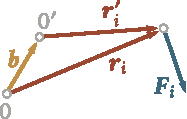
\includegraphics[scale=1]{figures/ch_05/fig_5_21.pdf}
			\caption[]{}
			\label{fig:5_21}
		\end{center}
	\end{minipage}
	\hspace{-0.05cm}
	\begin{minipage}[t]{0.7\linewidth}
		\begin{center}
			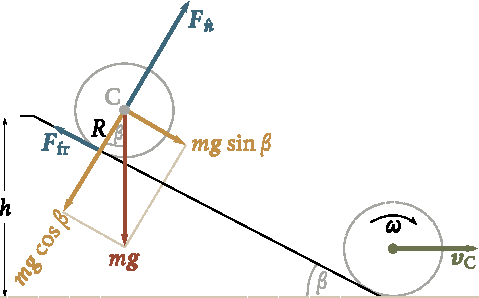
\includegraphics[scale=1]{figures/ch_05/fig_5_22.pdf}
			\caption[]{}
			\label{fig:5_22}
		\end{center}
	\end{minipage}
\end{figure}

%It must be noted that the vector condition~\eqref{eq:5_58} is equivalent to three scalar ones:
Ta lưu ý rằng điều kiện vector~\eqref{eq:5_58} sẽ tương đương với ba điều kiện vô hướng:
\begin{equation}\label{eq:5_60}
	\sum M_{x,\text{ext}} = 0 ,\quad \sum M_{y,\text{ext}} = 0 ,\quad \sum M_{z,\text{ext}} = 0.
\end{equation}

%Thus, the conditions of equilibrium of a rigid body are determined by Eqs.~\eqref{eq:5_57} and~\eqref{eq:5_58}, or by Eqs.~\eqref{eq:5_57} and~\eqref{eq:5_60}.
Như vậy các điều kiện cân bằng của vật rắn được xác định bằng những phương trình Eqs.~\eqref{eq:5_57} và~\eqref{eq:5_58}, hoặc bằng những phương trình  Eqs.~\eqref{eq:5_57} và~\eqref{eq:5_60}.

%In conclusion, let us consider an example of the application of the laws of dynamics of a rigid body. Assume that a homogeneous cylinder of radius $R$ and mass $m$ rolls down an inclined plane (\fig{5_22}). Góc nghiêng của mặt phẳng bằng without slipping. The angle of inclination of the plane is $\beta$ and its height is $h$ ($h\sim R$). The initial velocity of the cylinder is zero. We are to find the velocity of the centre of mass and the angular velocity of the cylinder at the moment when it reaches the horizontal section. We shall give two variants of the solution.
Cuối cùng, ta hãy xét một ví dụ về sự vận dụng các định luật động lực học của vật rắn. Giả sử một hình trụ đồng tính có bán kính $R$ và khối lượng $m$ lăn không trượt trên một mặt phẳng nghiêng (\fig{5_22}). Góc nghiêng của mặt phẳng bằng $\alpha$, còn độ cao $h$ ($h\sim R$). Vận tốc ban đầu của hình trụ là bằng không. Ta tìm vận tốc của khối tâm và vận tốc góc quay của hình trụ tại thời điểm hình trụ đi ra tới phần nằm ngang. Ta đưa ra hai các giải.

\textbf{Cách thứ nhất.} Hình trụ sẽ chuyển động dưới tác dụng của ba lực: lực $\vec{P}=m\vec{g}$, lực ma sát $\vec{F}_{\text{fr}}$, và áp lực pháp tuyến $\vec{F}_{\hatvec{n}}$ (\fig{5_22}). Gia tốc của hình trụ theo hướng pháp tuyến của mặt phẳng là bằng không. Do đó, áp lực pháp tuyến về module bằng thành phần pháp tuyến của lực $\vec{P}$, có độ lớn $mg\cos\alpha$. %The cylinder will move under the action of three forces---the force $\vec{P}=m\vec{g}$, the force of friction $\vec{F}_{\text{fr}}$, and the force of normal pressure $\vec{F}_{\hatvec{n}}$ (see Sec.~\ref{sec:2_12}. The acceleration of the cylinder in the direction of a normal to the plane is zero. Consequently, the magnitude of the force of normal pressure equals the normal component of the force $\vec{P}$ having the magnitude $mg\cos\beta$.

%Friction appears between the cylinder and the plane at the points of their contact. In the absence of slipping, these points of the cylinder are stationary (they form an instantaneous axis of rotation). Hence, the force of friction we are dealing with is a static force of friction. We know from See.~\ref{sec:2_10} that the static force of friction can range from zero to the maximum value $F_0$ that is determined by the product of the coefficient of friction and the force of normal pressure pressing the contacting bodie against each oalp ($F_0=fmg\cos\beta$). In the case under consideration, the force of friction takes on a value such that slipping will be absent. Slipping will be absent when the cylinder rolls along the plane provided that the linear velocity of the points of contact vanishes. This will occur, in turn, if the velocity of the centre of mass $v_{\text{C}}$ at each moment of time equals the angular velocity of rotation of the cylinder $\vec{\omega}$ multiplied by the radius of the cylinder $R$:
Sự ma sát giữa hình trụ và mặt phẳng xuất hiện tại các điểm tiếp xúc của chúng. Khi không có sự trượt các điểm này của hình trụ sẽ đứng yên (chúng tạo thành trục quay tức thời), do đó lực ma sát được nói đến là lực ma sát nghỉ. Từ~\ref{sec:2_10} ta biết rằng lực ma sát nghỉ có thể có độ lớn nằm trong phạm vi từ không đến giá trị cực đại $F_0$, trong đó $F_0$ được xác định bằng tích của hệ số ma sát với áp lực pháp tuyến ép các vật tiếp xúc với nhau ($F_0=fmg\cos\alpha$). Trong trường hợp đang xét lực ma sát nhận giá trị sao cho không có sự trượt. Khi hình trụ lăn trên mặt phẳng, sự trượt sẽ không có trong điều kiện mà vận tốc dài của các điểm tiếp xúc là bằng không, điều này lại được nghiệm đúng nếu vận tốc $v_{\text{C}}$ của tâm quán tính tại mỗi thời điểm bằng vận tốc góc quay $\vec{\omega}$ của hình trụ nhân với bán kính $R$ của hình trụ:
\begin{equation}\label{eq:5_61}
	v_{\text{C}} = \omega R.
\end{equation}

\noindent
%The acceleration of the centre of mass $a_{\text{C}}$ will accordingly equal the angular acceleration $\alpha$ multiplied by $R$:
Một cách tương ứng, gia tốc $a_{\text{C}}$ của khối tâm sẽ bằng gia tốc góc $\beta$ nhân với $R$.
\begin{equation}\label{eq:5_62}
	a_{\text{C}} = \alpha R.
\end{equation}

%If the force of friction needed to obey conditions~\eqref{eq:5_61} and~\eqref{eq:5_62} does not exceed the maximum value $F_0$, then the cylinder will roll down the plane without slipping. Otherwise rolling without slipping is impossible.
Nếu lực ma sát cần để thực hiện các điều kiện~\eqref{eq:5_61} và~\eqref{eq:5_62} không vượt qua giá trị cực đại $F_0$, thì hình trụ sẽ lăn không trượt. Trong trường hợp ngược lại thì sự lăn không trượt là không thể xảy ra.

%Equation~\eqref{eq:5_6} in the given case has the form
Phương trình~\eqref{eq:5_6} trong trường hợp này có dạng
\begin{equation*}
	m\vec{a}_{\text{C}} = m\vec{g} + \vec{F}_{\text{fr}} + \vec{F}_{\hatvec{n}}.
\end{equation*}

\noindent
%Projecting it onto the direction of motion, we get
Chiếu lên phương chuyển động ta được
\begin{equation}\label{eq:5_63}
	ma_{\text{C}} = mg\sin\beta - F_{\text{fr}}.
\end{equation}

%For a homogeneous cylinder rotating about an axis of symmetry, $\vec{L}=I\vec{\omega}$. Therefore, \eqn{3_118} can be written in the form
Đối với một hình trụ đồng tính quay xung quanh trục đối xứng thì $\vec{L}=I\vec{\omega}$. Do đó có thể viết phương trình \eqn{3_118} dưới dạng
\begin{equation}\label{eq:5_64}
	I\alpha = \sum M_z
\end{equation}

\noindent
%where $z$ is the axis of the cylinder [(xem \eqn{5_51}). Trong \eqn{5_64}  written relative to the axis of the cylinder, only the moment of the force of friction will differ from zero. The remaining forces including the resultant of the forces of inertia are directed through the axis of the cylinder. As a result, their moments relative to this axis equal zero. Thus, \eqn{5_64} will be written as follows:
trong đó $z$ là trục của hình trụ (xem \eqn{5_51}). Trong \eqn{5_64} được viết đối với trục của hình trụ thì chỉ có moment lực ma sát sẽ khác không. Các lực còn lại, trong đó có cả hợp lực quán tính, có hướng đi qua trục hình trụ vì rằng các moment của chúng đối với trục này là bằng không. Như vậy, phương trình \eqn{5_64} được viết như sau:
\begin{equation}\label{eq:5_65}
	I\alpha = R\,F_{\text{fr}}.
\end{equation}

\noindent
%Here $I$ is the moment of inertia of the cylinder relative to its axis equal to $mR^2/2$.
Ở đây $I$ là moment quán tính của hình trụ đối với trục của nó bằng $mR^2/2$.

%Equations~\eqref{eq:5_63} and~\eqref{eq:5_65} contain three unknown quantities, $F_{\text{fr}}$, $a_{\text{C}}$ and $\alpha$. The last two of them are related by \eqn{5_62} resulting from the absence of friction. By solving the system of equations \eqref{eq:5_62}, \eqref{eq:5_63}, and \eqref{eq:5_65}, we shall find (with account of the fact that $I=mR^2/2$) các giá trị của các đại lượng cần tìm:) the values of the required quantities:
Trong các phương trình~\eqref{eq:5_63} và~\eqref{eq:5_65} có chứa ba đại lượng chưa biết: $F_{\text{fr}}$, $a_{\text{C}}$ and $\alpha$. Hai đại lượng cuối được liên hệ bởi điều kiện \eqn{5_62}, suy ra từ sự vắng mặt của ma sát. Giải đồng thời các phương trình \eqref{eq:5_62}, \eqref{eq:5_63}, và \eqref{eq:5_65}, ta tìm được (có tính đến $I=mR^2/2$) các giá trị của các đại lượng cần tìm:
\begin{align}
	F_{\text{fr}} &= \frac{1}{3} m g \sin\beta, \label{eq:5_66}\\
	a_{\text{C}} &= \frac{2}{3} g \sin\beta, \label{eq:5_67}\\
	\alpha &= \frac{2}{3}\left(\frac{g}{R}\right)\sin\beta. \label{eq:5_68}
\end{align}

%Now that we know the value of the static force of friction needed for rolling down of the cylinder without slipping, we can find the condition at which this rolling is possible. For the cylinder to roll down without slipping, the force~\eqref{eq:5_66} must not exceed the maximum value of the static force of friction $F_0$ equal to $fmg\cos\beta$:
Bây giờ ta đã biết độ lớn của lực ma sát nghỉ cần thiết để lăn hình trụ không trượt, ta có thể tìm được điều kiện sao cho sự lăn như thế có thể xảy ra. Để lăn không trượt, lực~\eqref{eq:5_66} không được vượt quá giá trị cực đại của lực ma sát nghỉ $F_0$ bằng $kmg\cos\alpha$:
\begin{equation*}
	\frac{1}{3} mg\sin\beta \leqslant mg\cos\beta
\end{equation*}

\noindent
từ đó
\begin{equation*}
	\tan\beta \leqslant 3f.
\end{equation*}

\noindent
%Consequently, if the slope ($\tan\beta$) of the plane exceeds the triple value of the static coefficient of friction between the cylinder and the plane, rolling down cannot occur without slipping.
Do đó, nếu tan của góc nghiêng của mặt phẳng vượt quá ba lần độ lớn của hệ số ma sát nghỉ giữa hình trụ và mặt phẳng, thì sự lăn không trượt không thể xảy ra.

%From the constancy of $a_{\text{C}}$ [see \eqn{5_67}) suy ra rằng khối tâm của hình trụ chuyển động nhanh dần đều. Trong thời gian] it follows that the centre of mass of the cylinder moves with uniform acceleration. During the time $t_{\text{r}}$ that it rolls down, the cylinder travels the distance $h/\sin\beta$. In uniformly accelerated motion, the distance, acceleration, and time are related by the equation $s=at^2/2$. Introducing the value of $s$, we get
Từ sự không đổi của $a_{\text{C}}$ (xem \eqn{5_67}) suy ra rằng khối tâm của hình trụ chuyển động nhanh dần đều. Trong thời gian lăn $t_{\text{r}}$ hình trụ đi được quãng đường $h/\sin\alpha$. Trong chuyển động nhanh dần đều, quãng đường, gia tốc và thời gian được liên hệ bằng hệ thức $s=at^2/2$. Nếu thay thế giá trị $s$ ta thu được.
\begin{equation*}
	\frac{h}{\sin\beta} = \frac{1}{2}a_{\text{C}}t_{\text{r}}^2
\end{equation*}

\noindent
%whence, introducing the value of $a_{\text{C}}$ từ  from \eqn{5_67}, we have
từ đó nếu chú ý tới giá trị $a_{\text{C}}$ từ \eqn{5_67} ta đi tới công thức
\begin{equation*}
	t_{\text{r}} = \frac{1}{\sin\beta}\left(\frac{3h}{g}\right)^{1/2}.
\end{equation*}

\noindent
%This time, like $a_{\text{C}}$, does not depend on the mass and radius of the cylinder\footnote{This holds only for a homogeneous solid cylinder.}. It is determined only by the angle of inclination of the plane $\beta$ and the difference between the levels of its edges $h$.
Khoảng thời gian này, cũng như $a_{\text{C}}$, không phụ thuộc vào khối lượng và bán kính của hình trụ\footnote{Điều này chỉ đúng đối với một hình trụ đặc đồng tính}. Nó chỉ được xác định bằng góc nghiêng $\alpha$ của mặt phẳng và hiệu $h$ của chiều cao các mép của nó.

%The velocity of the centre of mass when the cylinder reaches the horizontal section will be
Vận tốc của khối tâm khi hình trụ đi ra tới phần nằm ngang sẽ bằng
\begin{equation*}
	v_{\text{C}} = a_{\text{C}}t_{\text{r}} = \left(\frac{4}{3}gh\right)^{1/2}
\end{equation*}

\noindent
%and the angular velocity of the cylinder will be
còn vận tốc góc của hình trụ
\begin{equation*}
	\omega = \alpha t_{\text{r}} = \frac{1}{R} \left(\frac{4}{3}gh\right)^{1/2}.
\end{equation*}

%We must note that the static force of friction does no work on the cylinder because the points of the cylinder which this force is applied to are stationary at each moment of time [see \eqn{3_16}].
Ta chú ý rằng lực ma sát nghỉ không thực hiện công trên hình trụ, vì điểm của hình trụ mà lực này đặt vào là không chuyển động tại mọi thời điểm (xem \eqn{3_16}).

%We find for the horizontal plane ($\beta=0$) by Eqs.~\eqref{eq:5_67} and~\eqref{eq:5_68} that the cylinder will travel without acceleration if it is first imparted a certain translational velocity and the corresponding (such that no slipping occurs) angular velocity. The motion will actually be retarded. This is due to the force of rolling friction which is directed so that its moment reduces the angular velocity $\omega$, while the force itself produces a corresponding (again such that no slipping will appear) retardation of the centre of mass. The force of rolling friction does negative work on a rolling body.
Đối với một mặt phẳng ngang ($\alpha=0$), theo các công thức~\eqref{eq:5_67} và~\eqref{eq:5_68} đã có thì nếu ban đầu truyền cho hình trụ một vận tốc góc tịnh tiến và thích hợp nào đó (sao cho không xảy ra sự trượt) thì nó sẽ chuyển động không có gia tốc. Thật ra chuyển động sẽ chậm dần. Độ giảm tốc này được gây bởi lực ma sát lăn có hướng sao cho moment của nó làm giảm vận tốc góc $\omega$, còn chính lực sẽ gây ra độ giảm vận tốc tương ứng (một lần nữa, sao cho không xảy ra sự trượt) của khối tâm. Lực ma sát lăn thực hiện trên vật một công âm.

%In solving the problem on the rolling of a cylinder down an inclined plane, we disregarded rolling friction.
Khi giải bài toán về sự lăn của một hình trụ trên một mặt phẳng nghiêng ta đã bỏ qua ma sát lăn.

\textbf{Cách giải thứ hai.} Vì lực ma sát không thực hiện công (bỏ qua ma sát lăn), nên năng lượng toàn phần của hình trụ là không đổi. Tại thời điểm ban đầu động năng bằng không, thế năng bằng $mgh$. Tại cuối quá trình lăn, thế năng bằng không, tuy nhiên động năng sinh ra bằng (xem \eqn{5_55}) %Since the force of friction does no work (we disregard rolling friction), the total energy of the cylinder remains constant. At the initial moment, the kinetic energy is zero, and the potential energy is $mgh$. At the bottom of the inclined plane, the potential energy vanishes but a kinetic energy appears equal to [see \eqn{5_55}]:
\begin{equation*}
	E_{\text{k}} = \frac{mv_{\text{C}}^2}{2} + \frac{I_{\text{C}}\omega^2}{2}.
\end{equation*}

%Since slipping is absent, $v_{\text{C}}$ and $\omega$ are related by the expression $v_{\text{C}}=\omega R$. Introducing $\omega=v_{\text{C}}/R$ and $I_{\text{C}}=mR^2/2$ into the expression for the kinetic energy, we get
Vì không có sự trượt nên $v_{\text{C}}$ và $\omega$ liên hệ với nhau bằng hệ thức $v_{\text{C}}=\omega R$. Thay thế $\omega=v_{\text{C}}/R$ và $I_{\text{C}}=mR^2/2$ vào biểu thức động năng, ta được:
\begin{equation*}
	E_{\text{k}} = \frac{mv_{\text{C}}^2}{2} + \frac{mv_{\text{C}}^2}{4} = \frac{3}{4}mv_{\text{C}}^2.
\end{equation*}

%The total energy at the beginning and end of rolling down the inclined plane must be the same:
Năng lượng toàn phần tại đầu và cuối quá trình lăn sẽ phải như nhau:
\begin{equation*}
	\frac{3}{4}m\,v_{\text{C}}^2 = mgh
\end{equation*}

\noindent
từ đó
\begin{equation*}
	v_{\text{C}} = \left(\frac{4}{3}gh\right)^{1/2}
\end{equation*}

\noindent
còn vận tốc góc
\begin{equation*}
	\omega = \frac{v_{\text{C}}}{R} = \frac{1}{R} \left(\frac{4}{3}gh\right)^{1/2}.
\end{equation*}

%Pay attention to how much simpler the second variant of solution is than the first one.
Hãy chú ý là cách giải thứ hai đơn giản hơn cách giải thứ nhất biết chừng nào.

\section{Con quay hồi chuyển}\label{sec:5_9}

%A gyroscope (or top) is a massive symmetrical body rotating with a great velocity about an axis of symmetry. We shall call this axis the axis of the gyroscope. It is one of the principal axes of inertia. Therefore, if it does not turn in space, the angular momentum is $\vec{L}=I\vec{\omega}$, where $I$ is the moment of inertia relative to the gyroscope axis. Let us now assume that the gyroscope axis rotates with a certain velocity $\vec{\omega}'$. In this case, the resultant rotation of the gyroscope occurs about an axis not coinciding with an axis of symmetry, and the direction of the vector $\vec{L}$ does not coincide with that of the gyroscope axis. If the angular velocity $\omega'$ of the axis is negligibly small in comparison with the angular velocity $\omega$ of the gyroscope itself, however ($\omega'\ll\omega$), then we may assume that the vector $\vec{L}$ is approximately equal to $I\vec{\omega}$ and is directed along the gyroscope axis. In this condition, rotation of the vector $\vec{L}$ and rotation of the gyroscope axis will be equivalent. We shall assume in the following that the condition $\omega'\ll\omega$ is obeyed.
Một vật nặng đối xứng quay với vận tốc lớn xung quanh trục đối xứng được gọi là một con quay hồi chuyển (hay con quay). Ta sẽ gọi trục này là trục của con quay hồi chuyển. Trục của con quay hồi chuyển là một trong những trục quán tính chính. Do đó nếu nó không quay trong không gian thì moment động lượng bằng $\vec{L}=I\vec{\omega}$, trong đó $I$ là moment quán tính chính đối với trục của con quay hồi chuyển. Bây giờ ta giả sử rằng trục của con quay hồi chuyển quay với một vận tốc $\vec{\omega}'$ nào đó. Trong trường hợp này sự quay tổng hợp của con quay hồi chuyển sẽ xảy ra xung quanh một trục không trùng với trục đối xứng, và hướng của vector $\vec{L}$ không trùng với hướng của trục con quay hồi chuyển. Tuy nhiên, nếu vận tốc quay của trục là $\omega'$ nhỏ không đáng kể so với vận tốc quay riêng $\omega$ của con quay hồi chuyển ($\omega'\ll\omega$) thì có thể coi một cách gần đúng $\vec{L}$ bằng $I\vec{\omega}$ và hướng dọc theo trục của con quay hồi chuyển. Trong điều kiện này sự quay của vector $\vec{L}$ và sự quay của trục con quay hồi chuyển sẽ tương đương với nhau. Dưới đây ta sẽ giả thiết điều kiện $\omega'\ll\omega$ được thoả mãn.

%When an attempt is made to turn the gyroscope axis, a distinctive phenomenon is observed called the gyroscopic effect: under the action of forces that ought to cause rotation of the gyroscope axis $00$ about straight line $0'0'$ (\fig{5_23}), the axis turns about straight line $0''0''$ (axis $00$ and straight line $0'0'$ are in the plane of the drawing, and straight line $0''0''$ and the forces $\vec{F}_1$ and $\vec{F}_2$ are at right angles to this plane). The behaviour of the gyroscope, which seems unnatural at first sight, completely conforms with the laws of rotational dynamics. Indeed, the moment of the forces $\vec{F}_1$ and $\vec{F}_2$ is directed along straight line $0'0'$. During the time $\deriv{t}$, the angular momentum of the gyroscope $\vec{L}$ receives the increment $\deriv{\vec{L}}=\vec{M}\,\deriv{t}$, which has the same direction as $\vec{M}$. After the time $\deriv{t}$ elapses, the angular momentum of the gyroscope will equal the resultant $\vec{L}'=\vec{L}+\deriv{\vec{L}}$ in the plane of the figure. The direction of the vector $\vec{L}'$ coincides with the new direction of the gyroscope axis. Thus, the latter will turn about straight line $0''0''$ through a certain angle $\deriv{\varphi}$. It can be seen from \fig{5_23} that $\deriv{\varphi}=|\deriv{\vec{L}}|/L=M\,\deriv{t}/L$. Hence, it follows that the gyroscope axis turned to its new position with the angular velocity $\omega'=\diffin{\varphi}{t}=M/L$. Let us write this relation in the form $M=\omega'L$. The vectors $\vec{M}$, $\vec{L}$ and $\vec{\omega}'$ are mutually perpendicular (the vector $\vec{\omega}'$ is directed along straight line $0''0''$ toward us). The relation between them can therefore be written in the form
Khi thử gây ra sự quay quanh trục con quay hồi chuyển thì người ta quan sát được một hiện tượng đặc thù có tên là \textbf{hiệu ứng con quay hồi chuyển}: dưới tác dụng của các lực mà có vẻ như chúng sẽ phải gây ra sự quay trục $OO$ của con quay hồi chuyển xung quanh đường thẳng $O'O'$ (\fig{5_23}), thì trục này quay xung quanh đường thẳng $O"O"$ (trục $OO$ và đường thẳng $O'O'$ được giả thiết nằm trong mặt phẳng hình vẽ, còn đường thẳng $O"O"$ và các lực $\vec{F}_1$ và $\vec{F}_2$ vuông góc với mặt phẳng này). Hành vi của con quay hồi chuyển thoạt nhìn ngược với tự nhiên là hoàn toàn phù hợp với các định luật động lực học của chuyển động quay. Thực vậy, moment của các lực $\vec{F}_1$ và $\vec{F}_2$ được hướng dọc theo đường thẳng $O'O'$. Trong khoảng thời gian $\deriv{t}$, moment động lượng $\vec{L}$ tăng được một khoảng $\deriv{\vec{L}}=\vec{M}\,\deriv{t}$ có cùng hướng như $\vec{M}$. Sau thời gian $\deriv{t}$, moment động lượng của con quay hồi chuyển sẽ bằng moment tổng $\vec{L}'=\vec{L}+\deriv{\vec{L}}$ nằm trong mặt phẳng hình vẽ. Hướng của vector $\vec{L}'$ sẽ trùng với hướng mới của trục con quay hồi chuyển. Như vậy trục của con quay sẽ quay xung quanh đường thẳng $O"O"$ một góc $\deriv{\varphi}$ nào đó. Từ hình \fig{5_23} rõ ràng là $\deriv{\varphi}=|\deriv{\vec{L}}|/L=M\,\deriv{t}/L$. Từ đây suy ra rằng sự quay trục con quay hồi chuyển tới vị trí mới đã xảy ra với vận tốc góc $\omega'=\diffin{\varphi}{t}=M/L$. Ta viết hệ thức này dưới dạng: $M=\omega'L$. Các vector $\vec{M}$, $\vec{L}$ và $\vec{\omega}'$ đều vuông góc với nhau (vector $\vec{\omega}'$ có hướng dọc theo đường thẳng $0''0''$ về phía người đọc). Do đó có thể viết mối liên hệ giữa chúng dưới dạng
\begin{equation}\label{eq:5_69}
	\vec{M} = \vec{\omega}' \times \vec{L}.
\end{equation}

\begin{figure}[!htb]
	\begin{minipage}[t]{0.55\linewidth}
		\begin{center}
			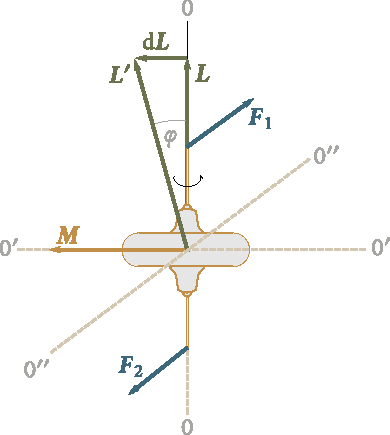
\includegraphics[scale=0.95]{figures/ch_05/fig_5_23.pdf}
			\caption[]{}
			\label{fig:5_23}
		\end{center}
	\end{minipage}
	\hspace{-0.05cm}
	\begin{minipage}[t]{0.45\linewidth}
		\begin{center}
			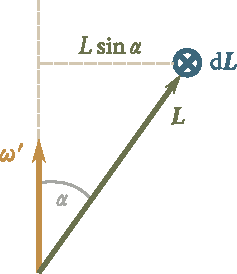
\includegraphics[scale=0.95]{figures/ch_05/fig_5_24.pdf}
			\caption[]{}
			\label{fig:5_24}
		\end{center}
	\end{minipage}
\end{figure}

\noindent
%We have obtained this equation for the case when the vectors $\vec{\omega}'$ and $\vec{L}$ are mutually perpendicular. It also holds, however, in the most general case. A glance at \fig{5_24} shows that when the gyroscope axis turns about the vector $\vec{\omega}'$ through the angle $\deriv{\varphi}$ the vector $\vec{L}$ receives an increment whose magnitude is $|\deriv{\vec{L}}|=L\sin\alpha\,\deriv{\varphi}$. At the same time $|\deriv{\vec{L}}|=M\,\deriv{t}$. Thus, $L\sin\alpha\,\deriv{\varphi}=M\,\deriv{t}$, whence $M=\omega'L\sin\alpha$. It is easy to see with the aid of \fig{5_24} that in this case \eqn{5_69} holds (the vectors $\vec{\omega}'$ and $\vec{L}$ are in the plane of the figure, the vector $\deriv{\vec{L}}$ is directed beyond the drawing and is therefore depicted by a circle with a cross in it). We remind our reader that \eqn{5_69} is correct only if $\omega'\ll\omega$.
Ta đã có được công thức này đối với trường hợp khi các vector $\vec{\omega}'$ và $\vec{L}$ vuông góc với nhau. Tuy nhiên nó cũng đúng trong trường hợp tổng quát nhất. Như đã thấy từ hình \fig{5_24}, khi quay trục con quay hồi chuyển xung quanh vector $\vec{\omega}'$ một góc $\deriv{\varphi}$, vector $\vec{L}$ nhận một số gia có module bằng $|\deriv{\vec{L}}|=L\sin\alpha\,\deriv{\varphi}$. Đồng thời $|\deriv{\vec{L}}|=M\,\deriv{t}$. Vậy $L\sin\alpha\,\deriv{\varphi}=M\,\deriv{t}$, từ đó $M=\omega'L\sin\alpha$. Nhờ hình \fig{5_24} dễ dàng thấy được rằng \eqn{5_69} trong trường hợp này là đúng (các vector $\vec{\omega}'$ và $\vec{L}$ nằm trong mặt phẳng hình vẽ, vector $\deriv{\vec{L}}$ hướng ra sau hình vẽ và do đó được biểu diễn bằng một vòng tròn nhỏ với dấu chữ chéo). Ta nhớ rằng \eqn{5_69} chỉ đúng trong trường hợp $\omega'\ll\omega$.

%When attempts are made to cause the axis of a gyroscope to turn in a given way, the so-called gyroscopic forces are set up owing to the \textbf{gyroscopic effect}. These forces act on the bearings in which the gyroscope axis rotates. For example, if gyroscope axis $00$ is forcibly turned about straight line $0'0'$ (\fig{5_25}), the gyroscope axis tends to turn about straight line $0''0''$. To prevent this rotation, the forces $\vec{F}_1'$ and $\vec{F}_2'$ acting from the side of the bearings must be applied to the gyroscope axis. According to Newton's third law, the gyroscope axis will act on the bearings with the forces $\vec{F}_1$ and $\vec{F}_2$, and the latter are exactly the gyroscopic forces. Upon forced turning of the gyroscope axis with the angular velocity $\vec{\omega}'$, the moment of the forces with which the bearings act on the axis is determined by \eqn{5_69}. The moment of the gyroscopic forces with which the axis acts on the bearings is
Với các ý định quay trục con quay hồi chuyển bằng cách đã cho, do hiệu ứng con quay nên sẽ xuất hiện các lực được gọi là các \textbf{lực hồi chuyển} tác dụng lên các ổ trục mà trong đó trục của con quay hồi chuyển quay. Chẳng hạn, khi quay cưỡng bức, trục của con quay hồi chuyển $OO$ xung quanh đường thẳng $O'O'$ (\fig{5_25}) thì trục con quay hồi chuyển lại có xu hướng quay quanh đường thẳng $O"O"$. Để ngăn ngừa sự quay này cần phải đặt vào trục con quay hồi chuyển các lực $\vec{F}_1'$ và $\vec{F}_2'$ tác dụng từ phía các ổ trục còn lại. Theo định luật Newton thứ ba, trục con quay hồi chuyển sẽ tác dụng lên các ổ trục các lực $\vec{F}_1$ và $\vec{F}_2$ mà chính chúng là các lực hồi chuyển. Khi quay cưỡng bức trục con quay hồi chuyển với vận tốc góc $\vec{\omega}'$, moment của các lực mà các ổ trục tác dụng lên trục được xác định bằng \eqn{5_69}. Moment của các lực hồi chuyển mà trục tác dụng lên các ổ trục bằng
\begin{equation}\label{eq:5_70}
	\vec{M}' = \vec{L}' \times \vec{\omega}.
\end{equation}

\begin{figure}[!htb]
	\begin{minipage}[t]{0.45\linewidth}
		\begin{center}
			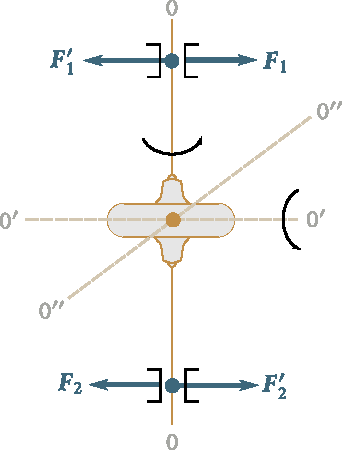
\includegraphics[scale=0.95]{figures/ch_05/fig_5_25.pdf}
			\caption[]{}
			\label{fig:5_25}
		\end{center}
	\end{minipage}
	\hspace{-0.05cm}
	\begin{minipage}[t]{0.55\linewidth}
		\begin{center}
			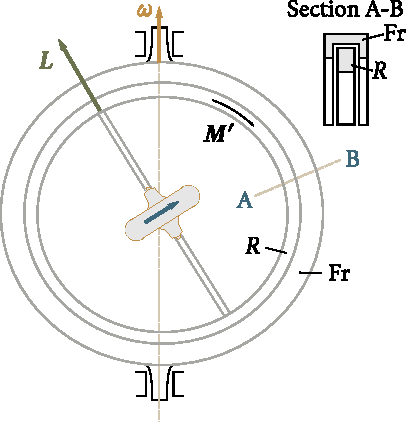
\includegraphics[scale=0.95]{figures/ch_05/fig_5_26.pdf}
			\caption[]{}
			\label{fig:5_26}
		\end{center}
	\end{minipage}
\end{figure}

%Let us assume that the axis of a gyroscope is fixed in ring $R$ that can freely turn in frame Fr (\fig{5_26}). Let us turn the frame about an axis in its plane with the angular velocity $\vec{\omega}'$. In this case, as we have found out, a moment of gyroscopic forces determined by \eqn{5_70} is produced that acts on the ring. This moment will cause the ring to turn in the frame in the direction indicated by the arrow until the gyroscope axis becomes arranged in the direction of the axis of rotation of the frame and the moment~\eqref{eq:5_70} vanishes. The direction of rotation of the gyroscope itself and the direction in which the frame turns will coincide. When $\vec{L}$ and $\vec{\omega}'$ are directed oppositely, the moment~\eqref{eq:5_70} also vanishes. The corresponding position of the gyroscope axis, however, will be unstable---upon the slightest deviation of the angle between $\vec{L}$ and $\vec{\omega}'$ from \SI{180}{\degree}, the moment $\vec{M}'$ will be set up that will turn the axis until this angle becomes equal to zero.
Giả sử rằng trục con quay hồi chuyển được đóng chắc vào vòng $K$ mà vòng này có thể quay tự do trong đai Ob (\fig{5_26}). Ta quay cái đai xung quanh trục nằm trong mặt phẳng của nó với vận tốc góc $\vec{\omega}'$. Trong trường hợp này, như ta đã giải thích, sẽ xuất hiện moment của các lực hồi chuyển được xác định bằng \eqn{5_70} tác dụng lên vòng. Dưới tác dụng của moment này vòng sẽ quay trong cái đai theo hướng mà mũi tên chỉ, cho tới khi trục của con quay hồi chuyển được định vị theo hướng của trục quay của cái đai và moment~\eqref{eq:5_70} trở nên bằng không. Khi đó hướng quay riêng của con quay hồi chuyển và hướng quay của cái đai trùng nhau. Khi $\vec{L}$ và $\vec{\omega}'$ hướng theo các hướng ngược nhau, thì moment~\eqref{eq:5_70} cũng bằng không. Tuy nhiên vị trí tương ứng của trục con quay hồi chuyển sẽ không bền, nghĩa là khi làm lệch góc giữa $\vec{L}$ và $\vec{\omega}'$ ra khỏi \SI{180}{\degree} một chút thì cũng đã xuất hiện một moment $\vec{M}'$ làm quay trục cho đến khi góc này trở nên bằng không.

\begin{figure}[!htb]
	\begin{center}
		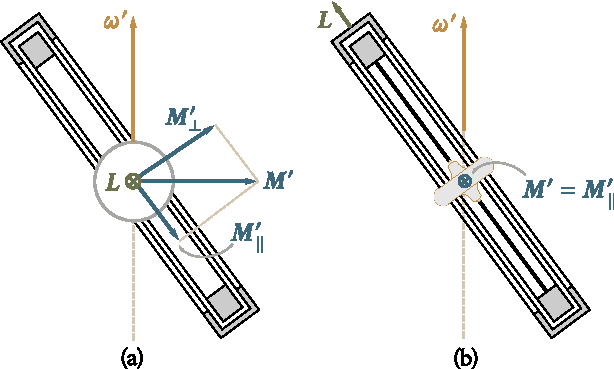
\includegraphics[scale=0.95]{figures/ch_05/fig_5_27.pdf}
		\caption[]{}
		\label{fig:5_27}
	\end{center}
\end{figure}

%Now let us assume that the frame turns with the angular velocity $\vec{\omega}'$ about an axis not in its plane (\fig{5_27}). In the position of the ring at which the angular momentum of the gyroscope $\vec{L}$ is perpendicular to $\vec{\omega}'$ (\fig{5_27}a), the vector $\vec{M}'$ has the direction shown in the figure. The component $\vec{M}_{\perp}'$ of this vector causes the ring to turn in the frame, and as a result the angle between the vectors $\vec{L}$ and $\vec{\omega}'$ will diminish. The component $\vec{M}_{\parallel}'$ tends to misalign the ring relative to the frame. When the ring occupies a position such that the angle between the vectors $\vec{L}$ and $\vec{\omega}'$ takes on the smallest possible value (\fig{5_27}b), the component $\vec{M}_{\perp}'$ will vanish because in this case the moment of the gyroscopic forces $\vec{M}'$ is in the plane of the ring; this moment cannot produce rotation of the ring in the frame. Thus, under the action of gyroscopic forces, the ring occupies such a position in the frame in which the angle between the gyroscope axis and the axis of rotation of the frame is minimum.
Bây giờ ta giả sử rằng cái đai quay với vận tốc góc $\vec{\omega}'$ xung quanh trục không nằm trong mặt phẳng của nó (\fig{5_27}). Tại vị trí của vòng mà moment động lượng $\vec{L}$ của con quay hồi chuyển vuông góc với $\vec{\omega}'$ (\fig{5_27}a), vector $\vec{M}'$ có hướng đã chỉ trên hình vẽ, Thành phần $\vec{M}_{\perp}'$ của vector này làm quay vòng quay trong cái đai, kết quả là góc giữa các vector $\vec{L}$ và $\vec{\omega}'$ sẽ giảm. Thành phần $\vec{M}_{\parallel}'$ có xu hướng làm lệch vòng đối với cái đai. Khi vòng chiến vị trí mà góc giữa các vector $\vec{L}$ và $\vec{\omega}'$ nhận giá trị khả dĩ nhỏ nhất (\fig{5_27}b) thì thành phần $\vec{M}_{\perp}'$ trở nên bằng không, vì trong trường hợp này moment $\vec{M}'$ của các lực hồi chuyển nằm trong mặt phẳng của vòng; moment này không thể làm quay vòng trong cái đai. Vậy dưới tác dụng của các lực hồi chuyển, vòng sẽ chiếm trong cái đai một vị trí mà tại đó góc giữa trục của con quay và trục quay của cái đai là cực tiểu.

\begin{figure}[!htb]
	\begin{minipage}[t]{0.4\linewidth}
		\begin{center}
			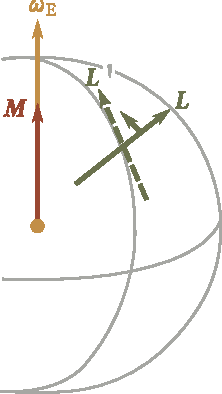
\includegraphics[scale=0.9]{figures/ch_05/fig_5_28.pdf}
			\caption[]{}
			\label{fig:5_28}
		\end{center}
	\end{minipage}
	\hspace{-0.05cm}
	\begin{minipage}[t]{0.6\linewidth}
		\begin{center}
			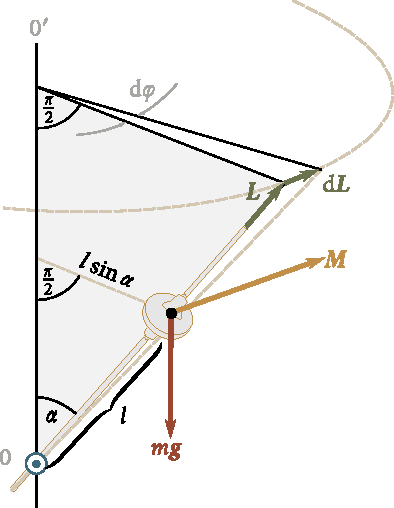
\includegraphics[scale=0.95]{figures/ch_05/fig_5_29.pdf}
			\caption[]{}
			\label{fig:5_29}
		\end{center}
	\end{minipage}
\end{figure}

%An instrument called the gyrocompass (gyroscopic compass) is based on the behaviour of a gyroscope described above. This instrument is a gyroscope whose axis can freely turn in a horizontal plane. The Earth's daily rotation causes the axis of the gyrocompass to arrange itself in a position such that the angle between this axis and the Earth's axis of rotation will be minimum (\fig{5_28}). In this position, the axis of the gyrocompass will be in a meridian plane and, consequently, line up in a north-south direction. A gyrocompass advantageously differs from its magnetic pointer counterpart in that no corrections have to be introduced into its readings for the so-called magnetic declination (the angle between the magnetic and the geographic meridians). Another advantage is that no measures have to be taken to compensate for the action on the pointer of ferromagnetic objects near the compass (for example, the steel hull of a ship).
Hành vi vừa được mô tả của con quay hồi chuyển là cơ sở của một dụng cụ được gọi là \textbf{la bàn hồi chuyển}. Dụng cụ này là một con quay hồi chuyển có trục có thể quay tự do trong một mặt phẳng nằm ngang. Dưới ảnh hưởng của sự quay suốt ngày đêm của Trái đất, trục của la bàn hồi chuyển được định vị vào vị trí mà tại đó góc giữa trục này và trục quay của Trái đất là cực tiểu (\fig{5_28}). Ở vị trí này, trục la bàn hồi chuyển nằm ở mặt phẳng kinh tuyến, và do đó chỉ đúng về phương Bắc. La bàn hồi chuyển có lợi hơn la bàn kim nam châm ở chỗ không cần phải đưa vào số chỉ của nó một sự hiệu chỉnh mà người ta gọi là độ từ thiên\footnote{Người ta gọi góc giữa kinh tuyến từ và kinh tuyến địa dư là độ từ thiên}, và cũng không cần đến các biện pháp để bù lại tác động lên kim của các vật sắt từ đặt gần nó (chẳng hạn như thân tàu bằng thép, v.v...)

%Assume that the axis of a gyroscope can freely turn about point $0$ (\fig{5_29}). Let us consider the behaviour of such a gyroscope in the field of forces of gravity. The magnitude of the moment of the forces applied to the gyroscope is
Giả sử rằng trục của con quay hồi chuyển có thể quay tự do quanh một điểm $O$ nào đó (\fig{5_29}). Ta khảo sát hành vi của một con quay hồi chuyển như thế trong trọng trường. Moment của các lực đặt vào con quay hồi chuyển về độ lớn sẽ bằng
\begin{equation}\label{eq:5_71}
	M = mgl\sin\alpha
\end{equation}

\noindent
%where $m$ is the mass of the gyroscope, $l$ is the distance from point $0$ to the centre of mass of the gyroscope and $\alpha$ is the angle made by the gyroscope axis with a vertical line.
trong đó $m$ là khối lượng của con quay hồi chuyển, $l$ là khoảng cách từ điểm $O$ đến khối tâm của con quay hồi chuyển, $\alpha$ là góc tạo bởi trục con quay hồi chuyển và đường thẳng đứng. Vector $\vec{M}$ được hướng vuông góc với mặt phẳng thẳng đứng đi quay trục của con quay (mặt phẳng này được tô đậm trên hình \fig{5_29}).

%The vector $\vec{M}$ is perpendicular to the vertical plane passing through the gyroscope axis (this plane is shaded in \fig{5_29}).

%Under the action of the moment $\vec{M}$, the angular momentum $\vec{L}$ changes during the time $\deriv{t}$ by the increment $\deriv{\vec{L}}=\vec{M}\,\deriv{t}$ perpendicular to the vector $\vec{L}$. The amount by which the vector $\vec{L}$ changes upon receiving the increment $\deriv{\vec{L}}$ corresponds to turning of the gyroscope axis such that the angle a does not change. The vertical plane passing through the gyroscope axis turns through the angle $\deriv{\varphi}$.4
Dưới tác dụng của moment $\vec{M}$ của các lực trong khoảng thời gian $\deriv{t}$, moment động lượng $\vec{L}$ nhận số gia $\deriv{\vec{L}}=\vec{M}\,\deriv{t}$ vuông góc với vector $\vec{L}$. Sự biến đổi của vector $\vec{L}$, bằng cách thu thêm số gia $\deriv{\vec{L}}$ sẽ tương ứng với sự quay trục con quay hồi chuyển, trong đó góc $\alpha$ không biến đổi. Khi đó mặt phẳng thẳng đứng đi qua trục con quay hồi chuyển quay một góc $\deriv{\varphi}$. Vector $\vec{M}$ cũng quay trong mặt phẳng ngang cùng một góc như thế. Kết quả là sau thời gian $\deriv{t}$ sẽ xảy ra sự sắp xếp tương hỗ của các vector $\vec{L}$ và $\vec{M}$ cũng giống như tại thời điểm đầu.

%The vector $\vec{M}$ turns through the same angle in a horizontal plane. As a result, when the time $\deriv{t}$ elapses, the vectors $\vec{L}$ and $\vec{M}$ will have the same mutual arrangement as at the initial moment.

%During the next moment $\deriv{t}$, the vector $\vec{L}$ again receives the increment $\deriv{\vec{L}}$ that is perpendicular to the new direction of the vector $\vec{L}$ setting in after the preceding elementary turn, etc. As a result, the gyroscope axis will rotate about the vertical axis passing through point $0$ with the angular velocity $\omega'$. It will describe a cone with an apex angle of $2\alpha$ (compare with \fig{5_24}). (When $\alpha=\pi/2$, the cone degenerates into a plane.) The vector $\vec{L}$ will change only in direction. Its magnitude will be constant because the elementary increments $\deriv{\vec{L}}$ will always be perpendicular to the vector $\vec{L}$\footnote{We can find similar behaviour in the velocity vector when a point moves uniformly along a circle. The vector $\vec{v}$ receives the increment $\deriv{\vec{v}}=\vec{a}_{\hatvec{n}}\,\deriv{t}$ ($\vec{a}_{\hatvec{n}}=\text{constant}$) during the time $\deriv{t}$. As a result, the direction of the vector $\vec{v}$ changes, while its magnitude remains constant.}.
Trong một thời gian nguyên tố $\deriv{t}$ tiếp theo, vector $\vec{L}$ lại nhận một số gia $\deriv{\vec{L}}$ vuông góc với hướng mới (xuất hiện sau sự quay nguyên tố xảy ra trước đó) của vector $\vec{L}$,v.v... Kết quả là trục con quay hồi chuyển sẽ quay xung quanh một trục thẳng đứng đi qua điểm $O$ với vận tốc góc $\omega'$ bằng cách vẽ một hình nón có góc mở bằng $2\alpha$ (so sánh với \fig{5_24}). (Với $\alpha=\pi/2$ hình nón suy biến thành một mặt phẳng). Khi đó vector $\vec{L}$ sẽ chỉ biến đổi về phương, còn về độ lớn nó sẽ không đổi, vì các số gia nguyên tố $\deriv{\vec{L}}$ sẽ luôn luôn vuông góc với vector $\vec{L}$\footnote{Vector vận tốc $\vec{v}$ trong chuyển động đều của một điểm trên một đường tròn cũng thể hiện một cách tương tự. Vector trong khoảng thời gian thu được một số gia $\deriv{\vec{v}}=\vec{a}_{\hatvec{n}}\,\deriv{t}$ ($\vec{a}_{\hatvec{n}}=\text{const}$). Kết quả là hướng của vector $\vec{v}$ bị biến đổi, còn độ lớn của nó lại không biến đổi.}.

%Thus, in the field of forces of gravity, the axis of a gyroscope with a fixed point rotates about a vertical line, describing a cone. Such motion of a gyroscope is called precession. We can find the angular velocity $\omega'$ of precession if we take into account that by \eqn{5_69} $M=\omega'L\sin\alpha$. Equating this value to \eqn{5_71}, we get $\omega'L\sin\alpha=mgl\sin\alpha$, whence
Vì vậy, trong trọng trường, trục con quay hồi chuyển có một điểm cố định sẽ quay xung quanh một đường thẳng đứng, bằng cách vẽ ra một hình nón. Chuyển động như vậy của con quay hồi chuyển được gọi là \textbf{sự tiến động}. Có thể tìm được vận tốc góc tiến động $\omega'$ nếu để ý rằng theo \eqn{5_69} $M=\omega'L\sin\alpha$. Cân bằng giá trị này với \eqn{5_71}, ta được $\omega'L\sin\alpha=mgl\sin\alpha$, từ đó
\begin{equation}\label{eq:5_72}
	\omega' = \frac{mgl}{L} = \frac{mgl}{I\omega}.
\end{equation}

\noindent
%It follows from \eqn{5_72} that the velocity of precession does not depend on the angle of inclination of the gyroscope axis with respect to a vertical line (on the angle $\alpha$).
Từ \eqn{5_72} suy ra vận tốc tiến động không phụ thuộc vào góc nghiêng của trục con quay hồi chuyển đối với đường thẳng đứng (góc $\alpha$).

\begin{figure}[!htb]
	\begin{center}
		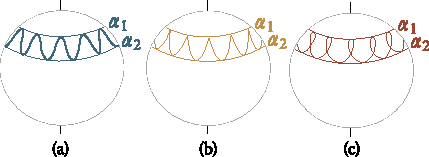
\includegraphics[scale=0.95]{figures/ch_05/fig_5_30.pdf}
		\caption[]{}
		\label{fig:5_30}
	\end{center}
\end{figure}

Cũng có thể thu được \eqn{5_72} như sau. Theo \fig{5_30}, góc quay $\deriv{\varphi}$ quay được trên mặt phẳng đi qua trục hình nón và trục con quay hồi chuyển có thể được biểu thị như tỉ số giữa $|\deriv{\vec{L}|}$ và $\vec{L} \sin \alpha$ (gốc của vector $\vec{L}$ được giả thiết đặt tại điểm $O$):
\begin{equation}\label{eq:5_72'}
    \deriv{\varphi}=\frac{|\deriv{\vec{L}}|}{\vec{L}\sin \alpha}=\frac{M\deriv{t}}{\vec{L}\sin\alpha}\frac{mgl\sin\alpha\deriv{t}}{M\sin\alpha}
\end{equation}
Rõ ràng rằng $\omega'=\deriv{\varphi}/\deriv{t}$. Chia biểu thức \eqn{5_72'} cho $\deriv{t}$, ta đi tới \eqn{5_72}.
%We have considered the approximate theory of the gyroscope. According to the strict theory, rotation of the axis about a vertical line is accompanied by oscillations of the axis in a vertical plane. The latter are attended by changes in the angle $\alpha$ ranging from $\alpha_1$ to $\alpha_2$. This wobbling of the axis is called \textbf{nutation}. Depending on the initial conditions, the end of a gyroscope axis draws one of the curves depicted in \fig{5_30} on an imaginary spherical surface. If, for example, after positioning the axis at the angle $\alpha_1$, we make the gyroscope rotate and then release the axis gently, the latter will first lower while rotating about the vertical line. After reaching the angle $\alpha_2$, the axis will begin to rise, and so on (this case is shown in \fig{5_30}b).
Ta đã nghiên cứu lý thuyết gần đúng về con quay hồi chuyển. Theo lý thuyết chặt chẽ thì, cùng với sự quay trục xung quanh đường thẳng đứng còn xảy ra các dao động của trục trong mặt phẳng thẳng đứng, kèm theo các sự biến thiên của góc $\alpha$ trong phạm vi từ $\alpha_1$ đến $\alpha_2$. Các dao động này của trục được gọi là \textbf{sự chương động}. Tuỳ theo các điều kiện ban đầu, đầu của trục con quay hồi chuyển sẽ vẽ trên mặt cầu tưởng tượng một trong các đường cong được mô tả trên hình \fig{5_30}. Chẳng hạn, nếu sau khi giữ chặt trục dưới một góc $\alpha_1$ rồi quay con quay hồi chuyển và sau đó buông trục ra nhẹ nhàng, thì thoạt tiên trục sẽ hạ xuống khi quay xung quanh đường thẳng đứng. Khi đạt tới góc $\alpha_2$ trục lại được nâng lên, v.v... (trường hợp này được mô tả trên hình \fig{5_30}b).

\begin{figure}[!htb]
	\begin{center}
		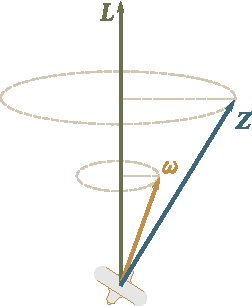
\includegraphics[scale=1.2]{figures/ch_05/fig_5_31.pdf}
		\caption[]{}
		\label{fig:5_31}
	\end{center}
\end{figure}

%By imparting an initial impetus of a quite definite magnitude and direction to a gyroscope, we can achieve precession of its axis without nutation. Such precession is defined as \textbf{regular}. The amplitude of nutation diminishes with an increasing gyroscope velocity of rotation. Nutation is also absorbed by friction in the support. This is why nutation is often unnoticeable in practice. Precession that is only approximately regular is called \textbf{pseudoregular}.
Nếu truyền cho con quay một cái đẩy ban đầu có độ lớn và hướng hoàn toàn xác định, thì có thể đạt được điều là trục con quay hồi chuyển sẽ tiến động không có chương động. Sự tiến động này được gọi là \textbf{tiến động đều đặn}. Con quay quay ngày càng nhanh thì biên độ chương động càng nhỏ. Ngoài ra, sự chương động bị khử bởi ma sát ở giá đỡ. Do đó trên thực tế sự chương động thường là không đáng kể. Sự tiến động chỉ gần đều đặn được gọi là \textbf{tiến động giả đều đặn}.

%If point $0$ is at the centre of mass of a gyroscope (see \fig{5_29}), the moment of the force of gravity becomes equal to zero, and we get the so-called free symmetrical top. Owing to the law of conservation, the angular momentum of such a top will change neither in magnitude nor in direction. If we rotate the top about its axis of symmetry, the vectors $\vec{L}$ and $\vec{\omega}$ will have the same direction which remains constant for an infinitely long time. If, however, the top is rotated about an axis not coinciding with any of its principal axes of inertia, the vectors $\vec{L}$ and $\vec{\omega}$ will not coincide (\fig{5_31}). The relevant calculations give us the following results. The vector $\vec{\omega}$ remains constant in magnitude and precesses about the direction of the vector $\vec{L}$ describing a cone. At the same time, the axis of symmetry $z$ of the top precesses, the vectors $\vec{L}$ and $\vec{\omega}$ and the $z$-axis constantly being in one plane. The top rotates about the $z$-axis with the angular velocity $\omega_z=L_z/I_z$, where $L_z$ is the projection of the vector $\vec{L}$ onto the $z$-axis, and $I_z$ is the moment of inertia of the top relative to this axis. The angular velocity of precession is $\omega_{\text{pr}}=L/I$, where $I$ is the identical value of the moments of inertia $I_x$ and $I_y$.
Nếu đặt điểm $O$ vào khối tâm của con quay hồi chuyển (xem \fig{5_29}) thì moment của trọng lực sẽ trở nên bằng không và ta có một con quay được gọi là \textbf{con quay đối xứng tự do}. Do định luật bảo toàn, moment động lượng của một con quay như thế sẽ không biến đổi cả về độ lớn lẫn về hướng. Nếu làm quay con quay xung quanh trục đối xứng, thì các vector $\vec{L}$ và $\vec{\omega}$ sẽ có hướng như nhau được giữ lâu mãi mãi. Tuy nhiên nếu con quay sẽ được làm quay xung quanh một trục không trục với một trục quán tính chính nào của nó thì các vector $\vec{L}$ và $\vec{\omega}$ sẽ không trùng nhau (\fig{5_31}). Sự tính toán thích hợp sẽ dẫn tới các kết quả sau. Vector $\vec{\omega}$ không thay đổi về độ lớn sẽ tiến động xung qunah hướng của vector $\vec{L}$, vạch ra hình nón. Đồng thời trục đối xứng $z$ của con quay sẽ tiến động, thêm vào đó các vector $\vec{L}$, $\vec{\omega}$ và trục $z$ luôn luôn nằm trong một mặt phẳng. Con quay quay xung quanh trục $z$ với vận tốc góc $\omega_z=L_z/I_z$, trong đó $L_z$ là hình chiếu của vector $\vec{L}$ lên trục $z$, $I_z$ là moment quán tính của con quay đối với trục này. Vận tốc góc tiến động bằng $\omega_{\text{pr}}=L/I$, trong đó $I$ là giá trị như nhau của các moment quán tính $I_x$ và $I_y$.
